\documentclass[a4paper,english,12pt,bibliography=totoc]{scrreprt}

\setlength{\parindent}{0pt} %no indentfirsts

\usepackage{amssymb}
\usepackage{tabularx}
\usepackage{graphicx}

\usepackage[T1]{fontenc} %immer
\usepackage[utf8]{inputenc} %am
\usepackage{babel} %Anfang

\usepackage{enumitem} %Aufzählungen verändern

%Gleichungen verwenden
\usepackage{newtxtext}
\usepackage{amsmath}
\usepackage{amssymb}
\usepackage{mathptmx}
%\usepackage{txfonts}

\usepackage{listings}% code blocks
\usepackage[most]{tcolorbox}

%Querverweise
\usepackage{varioref} %immer
\usepackage{hyperref} %in dieser
\usepackage{cleveref} %Reihenfolge

\usepackage{booktabs} %schönere Tabellen
\usepackage{siunitx} %SI-Einheiten
\usepackage{tabularx} %Tabellen mit flexiblen Spalten	

\usepackage{graphicx} %Grafiken verwenden
\usepackage{wrapfig}

\usepackage{lipsum} %Blindtext
\usepackage{subcaption}
\usepackage{afterpage}
\usepackage[headsepline]{scrlayer-scrpage} %Paket für Kopfzeilen
\usepackage{afterpage}
\usepackage{float}
\automark[subsection]{section}

\pagestyle{scrheadings}
\ihead{} % oben links
\chead{\leftmark} % oben Mitte
\ohead{} % oben rechts
\cfoot{\pagemark} % unten Mitte
\automark[section]{section} % Modified line

% Zu volle hboxen korrigieren
\tolerance 1414
\hbadness 1414
\emergencystretch 1.5em
\hfuzz 0.3pt
\widowpenalty=10000
\vfuzz \hfuzz
\raggedbottom

%Informationen über das Dokument
\date{\today}


\begin{document}


\begin{titlepage}
	\centering
	
\includegraphics[width=0.8\textwidth]{logo_uulm_sw}
	
	\vspace{1cm}
	\LARGE Laboratory Module for Master Programs
	\Huge \textbf{Biophysics Lab Course}
	
	\vspace{1cm}
	\Large Experiment:

	\Huge \textbf{Fluorescence Lifetime}
	
	\vspace{15mm}
	\Large Performed on 17.01.2024
	
	\vspace{5mm}
	\LARGE Group 8
	
	\vspace{1cm}
	\Large
	\begin{tabular}{rcl}
	\textbf{Haiyang Zhang} & and & \textbf{Nicolae Turcan}\\
	\href{mailto:student.1@uni-ulm.de}{haiyang.zhang@uni-ulm.de} & & \href{mailto:student.2@uni-ulm.de}{nicolae.turcan@uni-ulm.de}
	\end{tabular}
	
	\vspace{7mm}
	Supervisor: Umberto Seregni
	
	

\end{titlepage}



\tableofcontents

\chapter{Abstract}
\label{cha:abstract}

Fluorescence has become integral to biological sciences, playing a key role in biological imaging. This study focuses on fluorescence principles, such as fluorescence lifetime, and quantum yield. We also consider quenching mechanisms, including dynamic and static quenching, with dynamic quenching altering fluorescence lifetime and quantum yield, while static quenching affects signal intensity only.

Förster Resonance Energy Transfer (FRET), a nonradiative energy transfer mechanism, is discussed and studied, emphasizing its dependence on donor-acceptor distance which can be empolyed for nanometer-scale distance determination. Time-Correlated Single Photon Counting (TCSPC) is utilized to compute the fluorescence lifetime and  Instrument Response Function (IRF) is employed in bias correction.

The experiment involves studying Cy3, Cy3B, and Alexa647 dyes coupled with various forms of DNA to extract fluorescence lifetimes.The results highlight differences in dye properties and dye interactions. This study emphasizes the significance of fluorescence research for understanding molecular interactions.


\chapter{Introduction}
\label{cha:Introduction}
\begin{comment}
+ Cy3 and  Cy3B as molecules for lifetime measurements

+ Excited state and Relaxation with: Fluorescence/non-Radiative/FRET
+ Quantum Yield for Molecule
+ Fluorescence Lifetime
+ Dynamic Quenching and Static Quenching
+ Bleaching
+ FRET
-spectral overlap (Alexafluor647)
-distance (nanometric ruler)
-orientation (dipole-dipole coupling)
- Energy transfer efficiency( kinda Quantum Yield)

+Time-correlated single photon-coupling
-( signal * IRF)
\end{comment}


\begin{wrapfigure}{r}{0.45\textwidth}
  \centering
  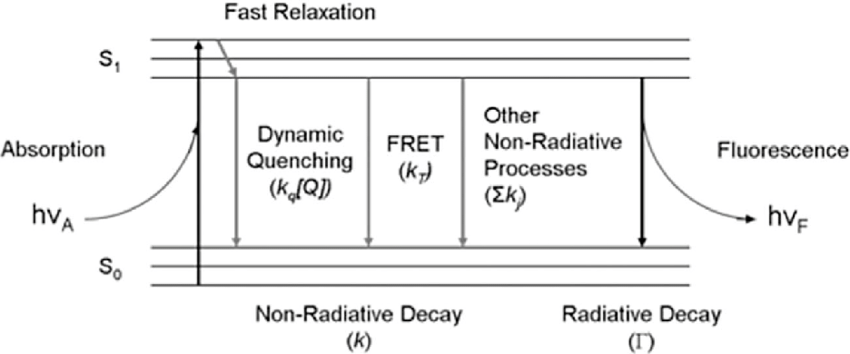
\includegraphics[width=0.44\textwidth]{images/other/A-simplified-Jablonski-diagram-illustrating-the-fluorescence-process-Photons-that-are.png}
  \caption{Jablonski diagram representing Radiative and Non-Radiative decays \hyperref[sec:ref_2]{[2]}.}
\end{wrapfigure}


During the past 15 years there has been a remarkable growth in the use of fluorescence in the biological sciences\hyperref[sec:ref_1]{[1]}. It is widely employed in biological imaging, medical diagnostics, and materials science for its ability to selectively illuminate and detect specific molecules or structures. The principle of fluorescence can be described using Jablonski diagram(Figure 2.1). A fluorophore could reach the excited singlet state $S_1$ by photon absorption( $\mathrm{hV_A}$ ), then it may return to the ground state $S_0$ by photon emission ( $\mathrm{hV_F}$ ))and nonradiative Decays ($\Gamma$ ) of which FRET is one of the possible decay pathways. 
\[
\mathrm{Fluorescence}: S_1 \stackrel{k_F}{\longrightarrow} S_0 + h\nu_F
\]
\[
\mathrm{Nonradiative}: S_1 \stackrel{k_{nr}}{\longrightarrow} S_0
\]
Here $k_F$ and $k_{nr}$ are rate constants. For a system has N molecules at excited state $S_1$, the depopulation of the excited state is described by the following differential equation:
\[
\frac{dN}{dt} = -k_F\cdot N - k_{nr}\cdot N
\]
with the solution of the equation
\[
N(t) = N(0)exp(\frac{-t}{\tau_F})
\]
Where the lifetime of excited state(also called fluorescence lifetime) $\tau_F$ is given by the inverse sum of all rate coefficients:
\[
\tau_F = \frac{1}{k_F+k_{nr}}
\]

The fluorescence quantum yield is the number of emitted photons over the number of absorbed photons, which equal to the ratio of fluorescent transitions over all possible deactivation processes. It could be written in the ratio of rate coefficients of the corresponding process:
\[
\phi_f = \frac{k_f}{k_f+k_{nr}}
\]

However, in the real reaction process, solvent molecules and the chemical environment will interact with the excited fluorophores and lead to energy changes. The reversible reduction of fluorescence due to an additional nonradiative process caused by interaction with a second molecule is called quenching. \\

The fluorescence quenching can be categorized into two types, dynamic quenching and static quenching. In dynamic quenching, the excited fluorophores collide with a quencher molecule and return to the ground state nonradiatively. This leads to a reduction in the fluorescence lifetime and fluorescence quantum yield, which is shown in the formulas below.
\[
\tau = \frac{1}{k_F+k_{nr}+k_Q[Q]} \qquad \qquad   \phi = \frac{k_F}{k_F+k_{nr}+k_Q[Q]}
\]
which depends on the quencher concentration [Q], and $k_Q$ is the quenching rate coefficient. The ratios of unquenched and quenched lifetime and quantum yields are given by :

\[
\frac{\tau_0}{\tau} = \frac{\phi_0}{\phi} =  1 + \tau_0k_Q[Q] = 1+ K_{sv}[Q]
\]
where $K_{sv}$ is the Stern-Volmer constant, which describes the concentration dependence of quenching.\\

In static quenching, fluorophores are captured in nonfluorescent complexes and become two species of fluorophores: nonfluorescent fluorophore/quencher complexes and free fluorophores with unaffected fluorescence. In this case, the fluorescence signal will decrease but the fluorescence lifetime will not change, because only free fluorophores will contribute to the lifetime measurement.\\

A special case of fluorescence quenching is Föster resonance energy transfer(FRET), the nonradiative energy transfer from an excited molecule(donor) to another fluorophore(acceptor) by dipole-dipole coupling. \\

There are several requirements that need to be fulfilled for FRET. First, the donor and acceptor fluorophores have to be in close proximity, which in general, is less than 10 nm. Additionally, the donor and acceptor dipole orientations must be approximately parallel. Furthermore, the emission spectrum of the donor has to overlap with the absorption spectrum of the acceptor, as is shown in figure 2.2. And the distance dependence of the rate coefficient for energy transfer is found to be:
\[
k_{FRET}(R) = \frac{1}{\tau_D}(\frac{R_0}{R})^6
\]
and
\[
R_0 = (\frac{9ln(10)\kappa^2\phi_DJ}{128\pi^5N_An^4})^{1/6}
\]
\\
Here $k_{FRET}$ is the rate coefficient of FRET, and $R_0$ is called Förster radius, which characterizes the FRET pair. The $\phi_D$ is the fluorescence quantum yield of the donor, n is the refractive index, $\kappa^2$ is the orientation factor, and J is the overlap integral, which is:
\[
J = \int \epsilon_A(\lambda)f_D(\lambda){\lambda}^4\, d\lambda
\]
For practical calculations, we use the following formula:
\[
R_0 = 0.0211(J\kappa^2n^{-4}\phi_D)^{1/6}
\]
\begin{figure}[H]
        \centering
        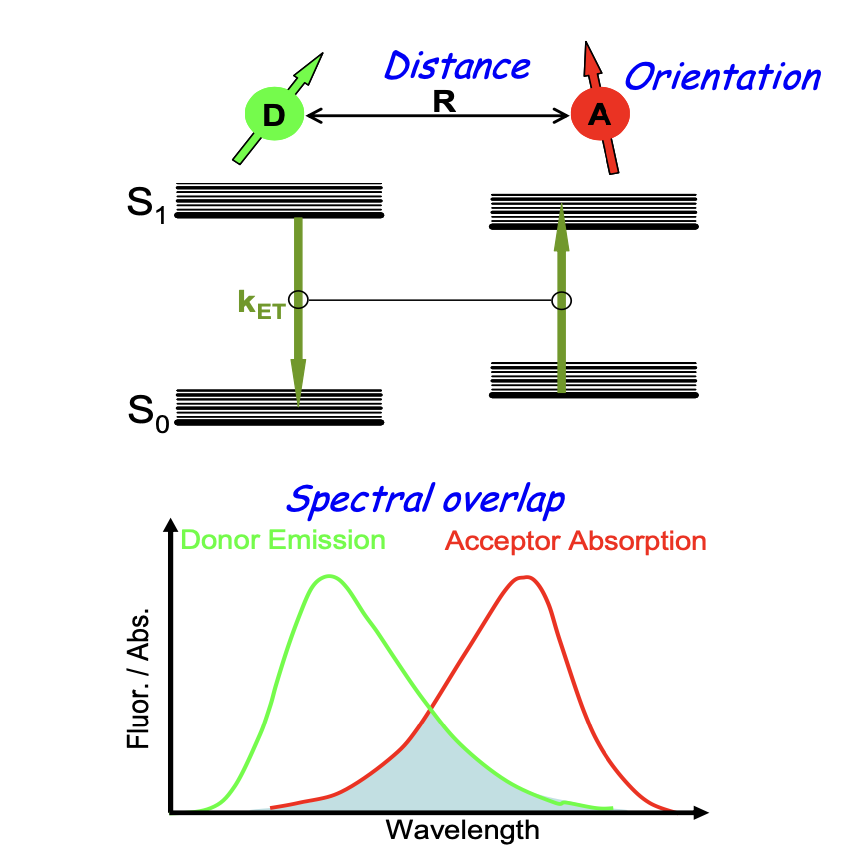
\includegraphics[width=0.9\textwidth]{images/other/FRET.png}
	    \caption{Steric and energetic conditions for efficient Föster transfer\hyperref[sec:ref_3]{[3]}}
\end{figure}

Here, the unit of the Föster radius is nm, while the unit of J is $(M \cdot cm)^{-1}$ and the wavelength in nm.\\

The energy transfer efficiency E is defined for the further calculation. When $R = R_0$, the efficiency should be 50\%. By definition, it is:
\[
E = \frac{k_{FRET}(R)}{k_{FRET}(R) + k_F + k_{nr}} = \frac{1}{1+(\frac{R}{R_0})^6}
\]
Because it is highly sensitive to the distance, FRET can be used to determine the distance around $R_0$ of the dye pair on the nanometer scale.\\

For the fluorescence lifetime studies, time-correlated single photon counting(TCSPC) is the most commonly used method. In this method, the arrival time of a photon is determined by the excitation laser pulse. A large number of photons were recorded to generate the stochastic distribution of arrival times, where each arrival time is represented by a bin in a histogram. In our particular case, we recorded photons until one of the bins reached 1500 photon counts. and for the simplest case, the fluorescence decay curve is a single exponential function with the decay constant equal to the fluorescence lifetime.\\

In practice, the exciting laser pulse is not infinitely short and the timing is not infinitely precise. Thus, an instrumental response function(IRF) is introduced. The IRF can be determined by measuring the nonfluorescent solution, and after the statistical correction using IRF, the exponential model function could finally be used to fit the fluorescence decay.\\


In our experiment, three types of dyes(Cy3, Cy3B, Alexa647) are applied for the fluorescence lifetime measurement. Theoretically, the intramolecular rotations due to the molecular structure of Cy3 will lead to a shorter fluorescence lifetime than Cy3B. The energy transfer of the FRET could also reduce the fluorescence lifetime of the donor molecules. Here, we investigate Cy3, Cy3B, and Cy3- and Cy3B- labelled DNA oligonucleotides.The primary objective is to investigate alterations in the local environment resulting from the attachment of DNA and its subsequent hybridization with a complementary DNA strand. Additionally, we aim to conduct a comprehensive analysis of FRET using an acceptor dye functionalized to the complementary strand. This will enable us to precisely determine the distance between the two labels within the double-stranded DNA structure.



\chapter{Material and Methods}
\label{cha:MaterialandMethods}

All the Materials were gently provided by our lab tutor and the University of Ulm, all the solutions were prepared beforehand and kept in 1.5 mL eppendorfs at -4 °C in a lab fridge, each sample was taken out only when used and thawed at hand temperature for a few minutes, the samples were gently shaken to avoid solute concentration gradients when pipetting.
The experiment with the restriction enzyme BamH was not performed by any of the laboratory groups because of time constraints. Solutions Cy3B and Cy3-ssDNA were low on stock, for this reason, we could perform only one measurement for each of the two samples.
We should also mention that the simple dye solutions couldn´t be distinguished based on their labels, but the experiment and the help of our lab tutor allowed us to distinguish between them based on their lifetimes.
\section{Material}
\label{sec:material}

This section contains the Materials used in the experiment.
Table 3.1 displays a list of the Laboratory equipment used to perform the experiment, the setup consisted of a washing and processing bench where the Quartz cuvette can be washed three times after each use, emptied and dried with clean Chemwipes, 2 distinct pipettes were used considering the difference in volumes handled, which were 72µL of PBS and 3µL of investigated solution.
Particular attention should be given to the optical instruments used to perform these measurements. 
The Quartz cuvette contained a volume of 75µL and was 3mm by 3mm in width and length. Quartz is the material of choice because of its purity ( only SiO2 without any additive ) and its refractive properties.
The cuvette has 3 clear surfaces and one black, so particular care was required when setting it inside the Fluorocube to avoid blocking the excitation or measurement faces.

The Fluorocube is a metal cube with the insides covered in a dark material to avoid reflections, it contains a metal stage for the Quartz cuvette and three side openings, and a top opening. The top opening is used to exchange the cuvette and the side openings are used as entry and exit points for the optical setup, in our case only two of the four openings are used, one for the excitation beam, and one for the lifetime measurements.
A NanoLed was used to create the excitation pulse, it has a repetition rate of a million times a second ( 1 MHz), and each pulse is only 1.2 nanoseconds long. The length of the pulse is required to be very short because we are interested in the photon emission after an excitation event, and fluorescence happens at this timescale. The repetition rate is this high because millions of events are required to create a fluorescence decay rate with significant for this stochastic process. 
The repetition rate of the NanoLed makes possible a time span between excitation events much longer than the excitation pulse, that allows to record single photon events
A monochromator is used to filter again the nanoLed pulse, the wavelength selected depends on the absorption peak of the fluorophore under analysis.
A lifetime sensor with nanosecond resolution was employed but we didn´t record any details regarding this instrument.

\begin{table}[htbp]
    \centering
    \begin{tabular}{|>{\raggedright}p{5cm}|p{7cm}|}
        \hline
        \textbf{Material} & \textbf{Details} \\
        \hline
        Phosphate Buffer Solution &  1µM \\
        \hline
        Deionized H2O &  In a wash bottle \\ 
        \hline
        Quartz Cuvette & 3mm$\times$3mm \\
        \hline
        Chemwipes & A box \\
        \hline
        Pipettes and Tips & 100µL, 10µL \\
        \hline
        Fluorocube & A dark stage for cuvette \\
        \hline
        NanoLed & 1MHz repetition rate, 1.2 ns pulse length \\
        \hline
        Monochromator & for excitation Wavelength \\
        \hline
        Lifetime Sensor & No details recorded \\
        \hline
        
    \end{tabular}
    \caption{Materials}
    \label{tab:materials_details}
\end{table}


The following table 3.2, contains the solutions that were used during this experiment.
As we stated above solutions Cy3B, and ssDNA-Cy3 were low on stock so only one measurement of their average lifetimes was performed.
The FretA and FretB solutions are labeled with Alexafluor-647 at the Thymines in position Y, the position of the label can be viewed in Fig. 3.1 .
We assumed that all the double strand DNA solutions contained only hybridized DNA and no single stranded DNA in solution.


\begin{table}[htbp]
    \centering
    \begin{tabular}{|>{\raggedright}p{4cm}|p{8cm}|}
        \hline
        \textbf{Solution} & \textbf{Details} \\
        \hline
        Cy3 & Dye in Methanol 1µM\\
        \hline
        Cy3B & Dye in Methanol 1µM\\
        \hline
        ssDNA-Cy3 & 5'-Cy3-labeled single-stranded DNA 1µM \\
        \hline
        ssDNA-Cy3B & 5'-Cy3B-labeled single-stranded DNA 1µM\\
        \hline
        dsDNA-Cy3 &  5'-Cy3-labeled double-stranded DNA 1µM\\
        \hline
        dsDNA-Cy3B & 5'-Cy3B-labeled double-stranded DNA 1µM\\
        \hline
        FretA & 5'-Cy3B-labeled double-stranded DNA and Alexa-647 bound in Y position 1µM\\ 
        \hline
        FretB & 5'-Cy3B-labeled double-stranded DNA and Alexa-647 bound in Y position 1µM\\
        \hline
    \end{tabular}
    \caption{Solutions Table and respective details}
    \label{tab:solutions}
\end{table}

In Figure 3.1 the sequences of the solutions ssDNA-Cy3, and ssDNA-Cy3B are defined as "Forward Cy3/Cy3B", it should be noted that position X corresponds to a Thymine labeled with Cy3B dye.
The solutions dsDNA-Cy3,dsDNA-Cy3B, FretA and FretB all contain a single strand described under "Forward Cy3/Cy3B", the complementary sequences are then described as "Reverse" for solutions dsDNA-Cy3 and dsDNA-Cy3B.
The complementary strands for the FRET samples are as suggested.

\begin{figure}[H]
        \centering
        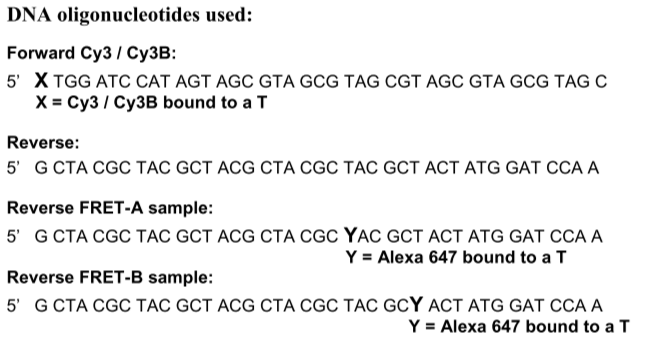
\includegraphics[width=0.8\textwidth]{images/other/DNAoligonucleotides_used.png}
	    \caption{Oligonucleotides sequences used in the solutions}
\end{figure}


\section{Methods}
\label{sec:methods}

The experimental procedures were divided into two main tasks. One team member focused on computational work at the dry bench, while the second team member was responsible for sample preparation at the wet lab bench, loading the samples into the Fluorocube to prevent potential contamination of the computer workspace.

After powering on the Fluorohub controller, TBX power supply, and the PC,the computational setup operated on Windows XP, afterwards the 'Datastation' software was launched. The 'TCSPC lifetime' mode was selected, and the 'R'eversed data option was chosen from the 'Tools' menu. Adjustments were made based on the emission spectrum of the dye and set to 500nm when recording the IRF and 570nm when recording the lifetime. For each measurement, the NanoLED output was activated from the 'NanoLED' panel, with particular attention to switching it of before opening the fluorocube. Each experiment involved recording two decays to ensure a more robust result.

For data analysis, the 'DAS6' software was utilized. The final output, including the lifetime decay, was saved in a .rtf file. Subsequently, these .rtf files were saved on a flash drive and used to extract the .png files presented in the results section of this report.

Additionally, Pymol was employed for molecular simulations to determine the distance between the Donor and Acceptor in both FretA and FretB.

\chapter{Experiment and Analysis}
\label{cha:experimenandanalysis}  



\section{Experiment}
\label{sec:experiment} 

\begin{comment}
    +describe why measuring the IRF is important
+describe the washing steps ( 3 times with a squeezing bottle containing ultra pure water to wash away all the molecules of the previous measurement) 
+describe the drying steps (with chem wipes, by holding the cuvette firmly and shaking it vigorously to push all the water out
+describe why cleaning the sides of the cuvette is important( to prevent alterations of the lifetime measurements and scratches that could worsen the efficiency of the optical setup)
+ describe how we added 72µL of PBS to the cuvette
+describe why measuring the IRF( Insturment response Function) is important( it helps in deconvolving the real signal from what the instrument creates)
+describe the importance of having someone at the computer to always set the right parameters,( to switch off the laser light, to save the files and figures, to initiate the analysis)
+describe why removing the sample from the fluorocube is important to prevent damage to the instrument( spilling inside an optical chamber)
+ describe why the samples are stored at 4c and why are taken out one by one ( photobleaching, damaging the DNA and creating multiple lifetime fractions that worsen the curve fit of the decay rate  )
+ describe that we agitated the epis to create a uniform sample and that this could be important to avoid very long recording times with the instruments( taking a portion of the solution on the top that has less molecules because they precipitated out of solution)
+ describe how careful handling is required when loading small volumes  such as the 3µL of sample ( 3µL are almost invisible to the naked eye and capillarity is extremely strong at this scale, making it possible to not load any sample at all)
+ describe how pipetting helped with mixing the solution in the quartz cuvette
+ describe how special attention was given when loading the cuvette in the measurement chamber( checking for the right orientation, and avoiding smudges on the cuvette sides by touching it only with chem wipes)
+ describe that there was variability in measurement times,( because it is based on reaching a certain photon count and some samples can be more efficient in emitting photons  than others)
+ describe how all the datasets  created were saved to allow future reference and the possibility for re-analysis
\end{comment}


The experiment consisted in replicating the method described above for all the samples in table 3.2. We replicated the experiment only two times and although two replicates are not enough to achieve any form of statistical significance for the resulting average lifetimes, more replicates were unfeasible because of the lack of resources and time.\\

For each replicate we paid close attention to the details to make sure we got accurate and reliable results.\\

Here's a breakdown of what we did:\\

\subsubsection{Cuvette Preparation}
We washed the quartz cuvette thoroughly before each lifetime measurement. Three rounds of rinsing with ultra-pure water from a squeezing bottle ensured that there were no leftover molecules from previous measurements, keeping our samples as consistent as possible.\\

After washing, we made sure the cuvette was completely dry using chem wipes. Giving it a firm and stron shake helped remove any remaining water droplets,that would change the final dilution of our sample, and make measurements extremely lengthy.\\
\subsubsection{Cleaning}
Cleaning the sides of the cuvette was also essential. Scratches on the cuvette could decrease the efficiency of our optical setup, so we took care to clean it from superficial smudges, debris and water droplets.\\
\subsubsection{Loading Procedure}
Following these preliminary preparation steps for the cuvette, we loaded 72µL of Phosphate Buffered Solution (PBS) into the cuvette with the 100µL pipette. \\
\subsubsection{Instrument Response Function (IRF) Measurement}
Measuring the Instrument Response Function (IRF) was a key step, because it allows us to extract the real photon arrival times from the recorded ones by comparing the IRF measured with PBS only with the real signal coming from PBS and sample. This step was crucial for interpreting our measurements accurately and not introduce a bias in our average lifetime that would make our results not comparable with known values.\\
\subsubsection{Task Division}
I underscore again how dividing the tasks into dry and wet allowed us to perform the measurements faster, with greater consistency and with less risks of contamination between the two benches.\\

One of us stayed at the computer throughout the experiment. They handled turning off the laser before loading the sample and back on before starting the measurement, and also saving files and figures with the appropriate names and details, and starting the analysis pipeline. This kept everything running smoothly.\\
\subsubsection{Sample Handling}
We ere particularly careful when loading and removing the samples from the from the Fluorocube. This prevented any damage to the instrument, like spillage inside the optical chamber.\\

To protect our samples from issues like photobleaching and dsDNA alterations (DNA melting resulting in the presence of ssDNA with a different lifetime), we stored them at -4°C and took them out one by one.\\
\subsubsection{Sample Preparation}
Before measurements, we agitated the eppendorf containing our sample, and pipetted from the bottom of the eppendorf to get a more uniform volume. In our opinion this helped avoid long recording times that could result from taking a portion of the solution with fewer molecules( near the solution meniscus as proper pipetting etiquette would suggest), which might have precipitated and thus created a concentration gradient.\\
\subsubsection{Pipetting Technique}
When loading small volumes, like the 3µL of sample, we were extra careful. These tiny amounts are almost invisible, and capillarity is super strong at this scale, so we needed to be precise with our pipetting, thus we used the 10µL pipette. Pipetting wasn't just about getting the right volume; it also helped mix the sample in the quartz cuvette. This made sure our measurements were consistent.\\
\subsubsection{Cuvette Handling}
Loading the cuvette into the measurement chamber needed attention. We checked its orientation to prevent the black side of the cuvette to be in the optical pathway, we also avoided smudges on the sides by using chem wipes when handling it.\\
\subsubsection{Measurement Variation}
Measurement times varied because it depended on reaching 1500 photons peak count, and some samples were more efficient at emitting photons than others. This could be because of various reasons that will be discussed more in detail in the following discussion chapter.\\
\subsubsection{Data Management}
Finally, we saved all our datasets for future reference and possible re-analysis. This should help in making our study more reproducible and transparent.
\\
The table 4.1 allows us to visualize a summary of the Experiments we performed, and it helped us keeping track of what steps where done before moving on, such a table can prove very useful when repeating the same experiment multiple times and we suggest adding it in some form for future laboratory manuals.\\

The columns represent the samples on which we performed the experiment, with the relative replicate. A checkmark or X can be used to record the outcome of the step. The titles are shorter for convenience in fitting the table in this report and the meaning of each title can easily be associated with the solutions described in the Materials section in table 3.2.


\begin{table}[h]
\centering
\resizebox{\textwidth}{!}{%
\begin{tabularx}{\textwidth}{|l|X|X|X|X|X|X|X|X|X|X|X|X|X|X|X|X|}
\hline
\textbf{Steps} & \multicolumn{2}{c|}{\textbf{Cy3}} & \multicolumn{2}{c|}{\textbf{Cy3B}} & \multicolumn{2}{c|}{\textbf{ssCy3}} & \multicolumn{2}{c|}{\textbf{ssCy3B}} & \multicolumn{2}{c|}{\textbf{dsCy3}} & \multicolumn{2}{c|}{\textbf{dsCy3B}} & \multicolumn{2}{c|}{\textbf{FrA}} & \multicolumn{2}{c|}{\textbf{FrB}} \\
\hline
Replicates & \#1 & \#2 & \#1 & \#2 & \#1 & \#2 & \#1 & \#2 & \#1 & \#2 & \#1 & \#2 & \#1 & \#2 & \#1 & \#2 \\
\hline
Empty Cuvette & $\checkmark$ & $\checkmark$ & $\checkmark$ & X & $\checkmark$ & X & $\checkmark$ & $\checkmark$ & $\checkmark$ & $\checkmark$ & $\checkmark$ & $\checkmark$ & $\checkmark$ & $\checkmark$ & $\checkmark$ & $\checkmark$ \\
\hline
Wash Cuvette & $\checkmark$ & $\checkmark$ & $\checkmark$ & X & $\checkmark$ & X & $\checkmark$ & $\checkmark$ & $\checkmark$ & $\checkmark$ & $\checkmark$ & $\checkmark$ & $\checkmark$ & $\checkmark$ & $\checkmark$ & $\checkmark$ \\
\hline
Dry Cuvette & $\checkmark$ & $\checkmark$ & $\checkmark$ & X & $\checkmark$ & X & $\checkmark$ & $\checkmark$ & $\checkmark$ & $\checkmark$ & $\checkmark$ & $\checkmark$ & $\checkmark$ & $\checkmark$ & $\checkmark$ & $\checkmark$ \\
\hline
Clean Sides & $\checkmark$ & $\checkmark$ & $\checkmark$ & X & $\checkmark$ & X & $\checkmark$ & $\checkmark$ & $\checkmark$ & $\checkmark$ & $\checkmark$ & $\checkmark$ & $\checkmark$ & $\checkmark$ & $\checkmark$ & $\checkmark$ \\
\hline
Load PBS & $\checkmark$ & $\checkmark$ & $\checkmark$ & X & $\checkmark$ & X & $\checkmark$ & $\checkmark$ & $\checkmark$ & $\checkmark$ & $\checkmark$ & $\checkmark$ & $\checkmark$ & $\checkmark$ & $\checkmark$ & $\checkmark$ \\
\hline
Record IRF & $\checkmark$ & $\checkmark$ & $\checkmark$ & X & $\checkmark$ & X & $\checkmark$ & $\checkmark$ & $\checkmark$ & $\checkmark$ & $\checkmark$ & $\checkmark$ & $\checkmark$ & $\checkmark$ & $\checkmark$ & $\checkmark$ \\
\hline
Load Sample & $\checkmark$ & $\checkmark$ & $\checkmark$ & X & $\checkmark$ & X & $\checkmark$ & $\checkmark$ & $\checkmark$ & $\checkmark$ & $\checkmark$ & $\checkmark$ & $\checkmark$ & $\checkmark$ & $\checkmark$ & $\checkmark$ \\
\hline
Record lifetime & $\checkmark$ & $\checkmark$ & $\checkmark$ & X & $\checkmark$ & X & $\checkmark$ & $\checkmark$ & $\checkmark$ & $\checkmark$ & $\checkmark$ & $\checkmark$ & $\checkmark$ & $\checkmark$ & $\checkmark$ & $\checkmark$ \\
\hline
\end{tabularx}%
}
\caption{Experiment Tracking}
\label{tab:my_label}
\end{table}

One last experiment was reported in the laboratory manual, the experiment consisted in treating sample FretB with a restriction enzyme that would cut the DNA, and record the lifetimes at 5 different timesteps ( t0 = 0, t1= 5 min, t2= 10 min, t3= 20 min, t4= 30 min).
This experiment was not performed because of time constraints.
We assume that this experiment was supposed to show an increase in average fluorescence, increasing as the incubation time became longer until stabilizing when all the donor-only species ( Cy3B attached to a Thymine) would be completely free to float away from the acceptor (Alexafluor 647 attached to a thymine in Y position).

\section{Data Analysis}
\label{sec:analysis} 

In the analysis of Fluorescence Lifetime experiments, we utilized DAS6, a specialized software for data analysis, to perform the statistical analysis of the lifetime decay histogram. Each measurement underwent a curve fit to analyze which lifetime decay rate best fitted the data effectively. By setting specific parameters, such as known lifetimes of fractions of the sample we were able to achieve better fitting results. as was the case for the Fret experiments. Both our lab tutor and experimental results indicated that curve fittings with residuals of high significance( standard deviation above 4) we still considered to be acceptable results.\\

The DAS6 output window , which can be viewed in many of the figures in the appendix, shows a lifetime decay histogram displayed with fitted curves. Various Parameters and their values are listed on the right side of the window. Below the histogram, there is another graph displaying residuals.\\

The statistics involved in this process include curve fitting and the R-value ( described under Chi-Squared since we used it for testing model assumptions rather than predictions, where the assumption is that the distribution of fluorescence lifetimes follow an exponential decay function). Curve fitting is a type of statistical analysis used to ensure that data points align as closely as possible with a curve to represent them accurately. The R-value indicates how well the curve fits the data points; a higher R-value suggests a better fit.\\

To delve deeper into curve fitting, it is a process in statistics where the goal is to construct a curve, or mathematical function, that has the best fit to a series of data points ( our recorded histogram of photon arrival times).





\chapter{Results and Discussion}
\label{cha:ResultsandDiscussion}

\section{Results}
\label{sec:Results} 


\begin{comment}
    +Determine the fraction of "Donor Only Species from relative amplitude"
+Determine lifetime of fluorescence lifetime of Cy3B in presence of the Acceptor
+Calculate FRET efficiency for FretA and FretB
+Determine distance of the dyes assuming a Forster Radius of 6.8nm for FretA and FretB
+ Calculate the expected distances using the knowledge of the dna sequences in both( done by Nicolai in Pymol if he manages or simply calculated approximating the length of each aminoacid to X nm)
+ Compare the results of computed vs real distance


+ All the screenshots of the results with a title and a short discussion on how many populations we expect in the solution,( ex dsDNACy3B solution could be composed of: FreeCy3B, ssDNACy3B and dsDNACy3B), what issues we encountered (long vs short recording times and why that could be) and a comment on the Std. deviation of the real values from the FIT, (if they are more than +-4 , that it could mean we have multiple lifetimes recorded simultaniously)

\end{comment}
In the experiment, we acquired the TCSPC curves of IRF and different samples(see Table 3.2). The fluorescence lifetime of the fluorophores was obtained by curve fitting. For FRET samples, we can calculate the FRET efficiency and relative amplitudes using the fitting results. The answers to the problems on the script are as follows.\\

The following Table 5.1 the average lifetimes expressed in nanoseconds for each sample replicate are presented, as we can see the difference in average lifetimes recorded for each replicate are negligible.


\begin{table}[h]
\centering
\begin{tabular}{|l|c|c|}
\hline
\textbf{Samples} & \multicolumn{2}{c|}{\textbf{Lifetimes (ns)}} \\
\hline
Cy3 & 0.34 & 0.32 \\
\hline
Cy3B & 2.37 & x.xx \\
\hline
ssCy3 & 1.23 & x.xx \\
\hline
ssCy3B & 2.92 & 2.85 \\
\hline
dsCy3 & 1.69 & 1.64 \\
\hline
dsCy3B & 2.91 & 2.90 \\
\hline
FRET A & 1.34 & 1.38 \\
\hline
FRET B & 0.68 & 0.66 \\
\hline
\end{tabular}
\caption{Recorded Lifetimes for Sample Replicates}
\label{tab:lifetimes}
\end{table}



\subsection{Preliminaries}
\begin{figure}[H]
        \centering
        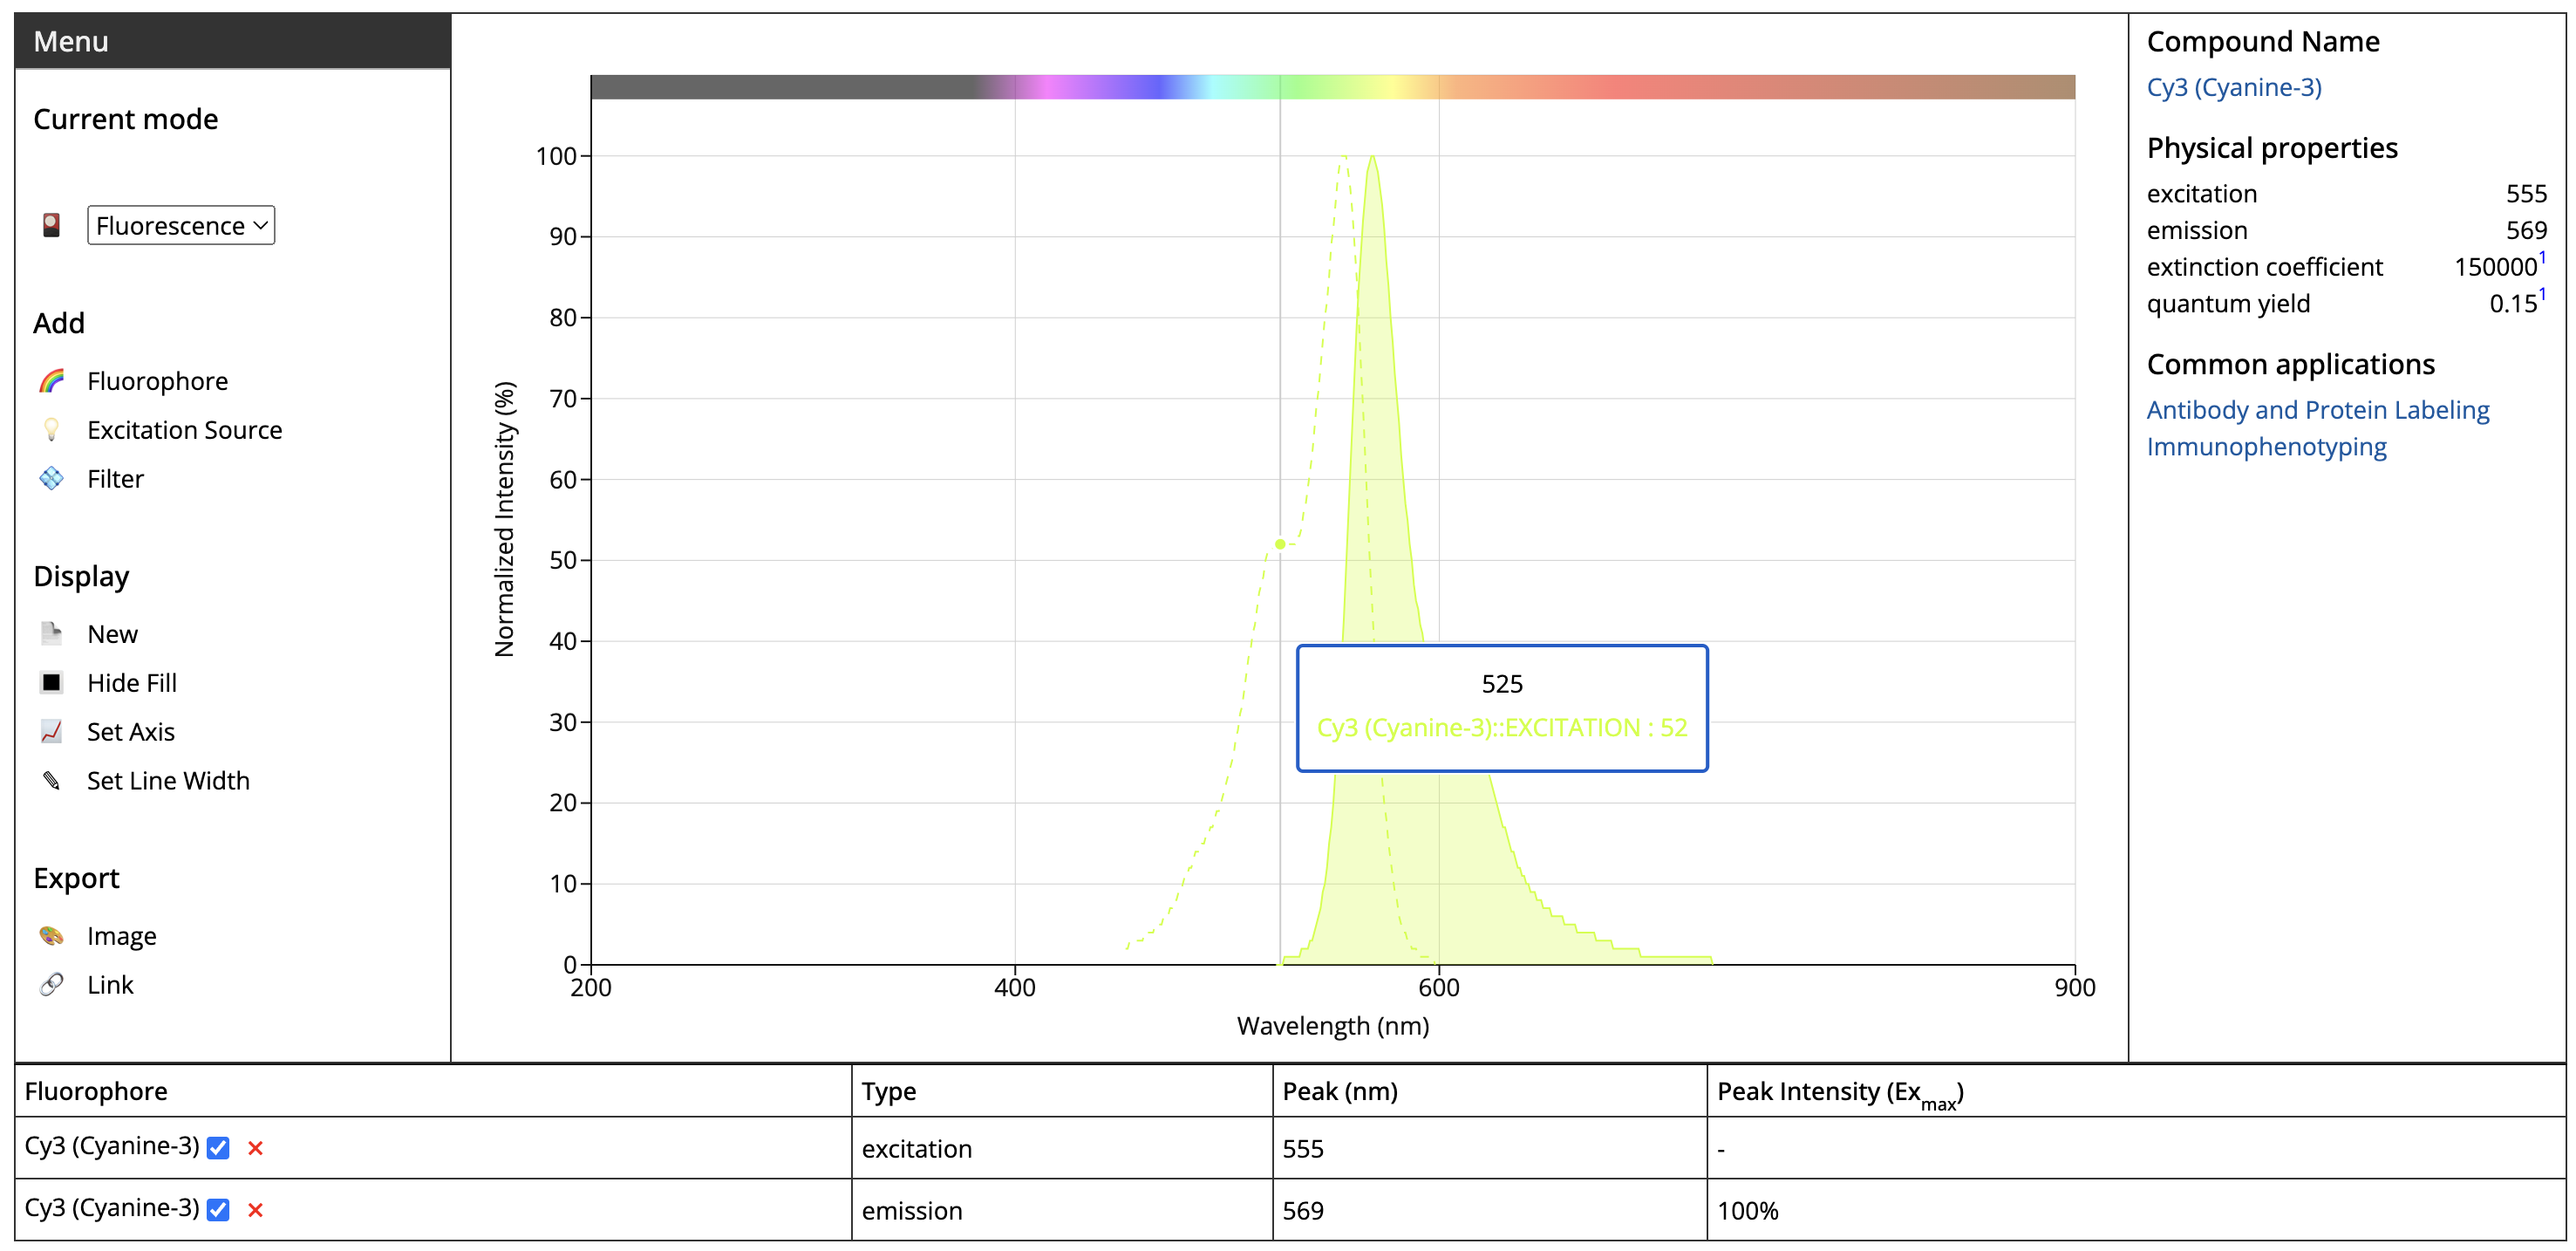
\includegraphics[width=0.9\textwidth]{images/other/Cy3_properties.png}
	    \caption{The excitation and emission spectrum of Cy3\hyperref[sec:ref_4]{[4]}}
\end{figure}
The excitation and emission spectrum is shown in the figure 5.1. From the spectrum, we can obtain that the wavelength of the emission peak is at 569nm. This wavelength could help us to determine where should we detect the emission photons. Besides, the left boundary of the overlap on the excitation and emission spectrum could be a reference for us to set the wavelength of the laser.\\

The IRF can be determined by performing the TCSPC measurements on the PBS buffer. For each sample, the IRF should be measured independently.\\

\subsection{IRF and dye measurements}
In figure 7.1, 7.2 and 7.3(see Appendix), the IRF was detected at the wavelength of 500 nm. And by curve fitting and calculate the average fluorescence lifetime aquired from two attempts(only once for the Cy3B), the fluorescence lifetime of the dyes Cy3 in PBS is $3.25 \times 10^{-10}s$ %(standard deviation~$4\times 10^{-12}s$)
, and for dyes Cy3B, the fluorescence lifetime in PBS is $2.38 \times 10^{-9}s$ %(standard deviation = $6.89 \times 10^{-12}s$)
. 

\begin{comment}
    
\begin{figure}[H]

    \begin{subfigure}{0.45\textwidth}
        \centering
        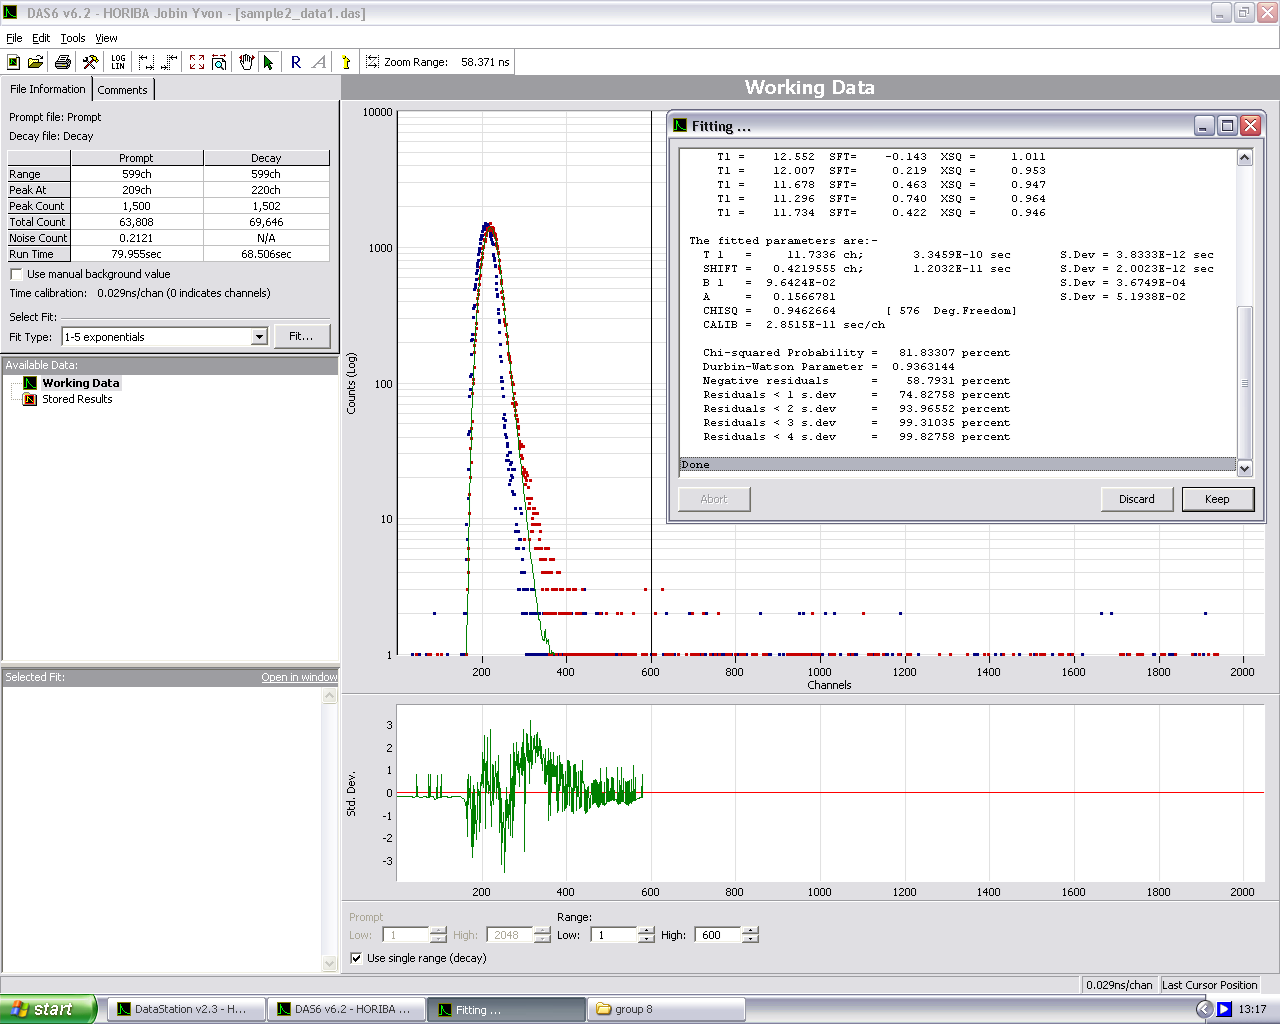
\includegraphics[width=\textwidth]{images/dyes/Cy3_data1_fit1.png}
        \caption{TCSPC curve and the fitting of the first group of Cy3}
    \end{subfigure}
    \begin{subfigure}{0.45\textwidth}
        \centering
        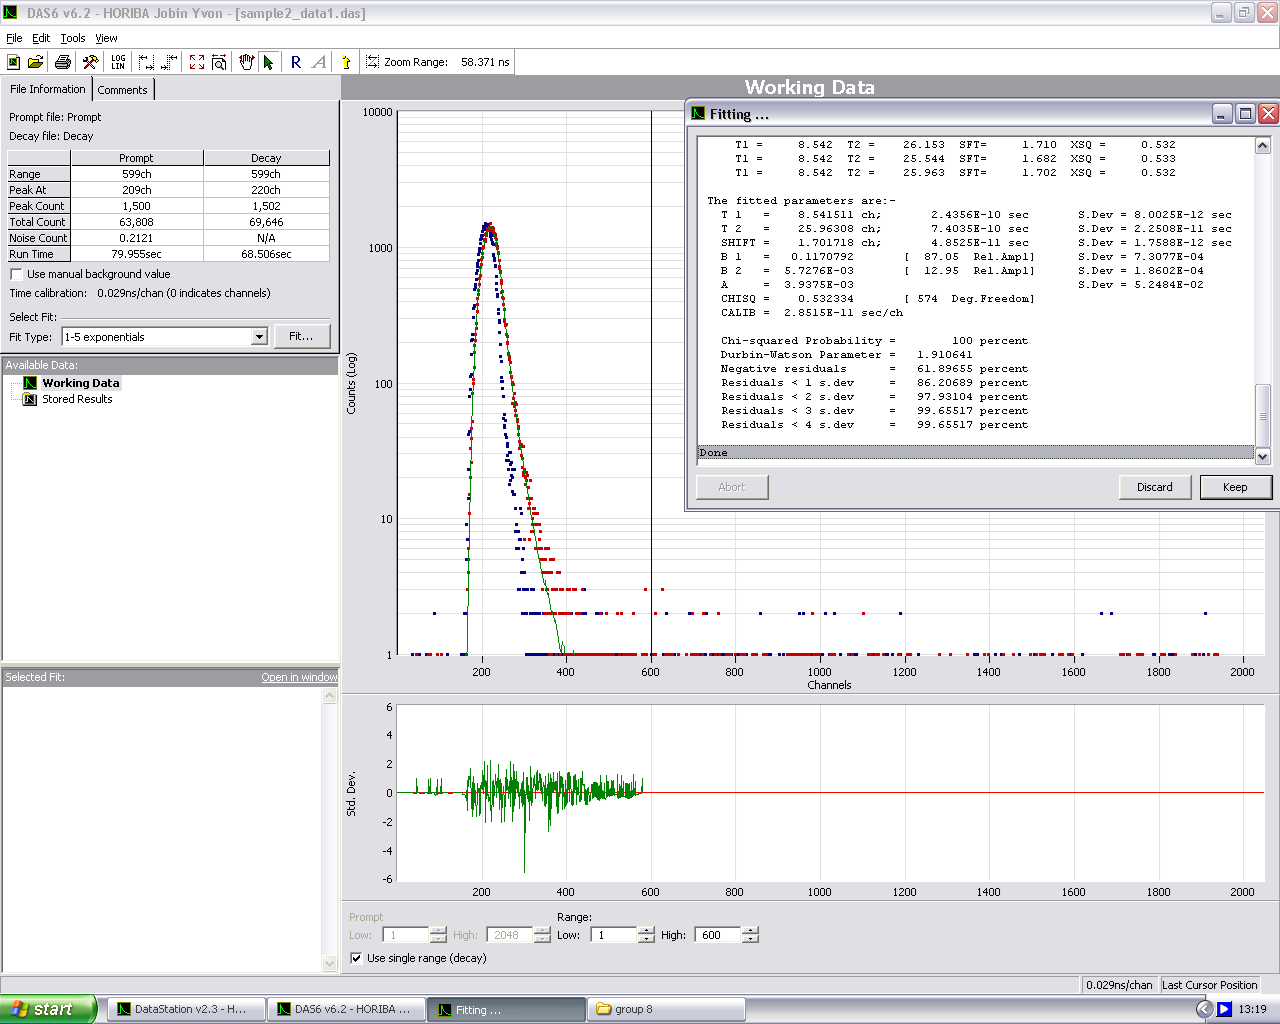
\includegraphics[width=\textwidth]{images/dyes/Cy3_data1_fit2.png}
        \caption{TCSPC curve and the fitting of the first group of Cy3}
    \end{subfigure}
    \caption{}
    
\end{figure}
\end{comment}
\subsection{Fluorescence lifetime for structure sensing}
The curves and fitting results of the TCSPC measurements on 5'-Cy3-labeled single-stranded DNA are shown in figure 7.4 and (see Appendix). Applying the single exponential fitting, we acquired the fluorescence lifetime of Cy3-labeled single stranded DNA is $1.23 \times 10^{-9}s$ %(standard deviation $1.22 \times 10^{-11}s$)
.\\

For the molecules has the same construct but hybridized to a complementary DNA(figure 7.7 and 7.8), the fluorescence lifetime is $1.37 \times 10^{-9}s$ %(standard deviation ~$9 \times 10^{12}$)
. Comparing with the Cy3 labeled single-stranded DNA, the fluorescence lifetime is slightly longer.\\

And as for the single-stranded(figure 7.5 and 7.6) and double-stranded DNA (figure 7.9 and 7.10) labeled by Cy3B, the fluorescence lifetimes are $2.89 \times 10^{-9}s$ %(standard deviation~$7.5\times 10^{-12}s$)
and $2.89 \times 10^{-9}s$ %(standard deviation~$6.9 \times 10^{-12}s$)
.  Analyzing these four groups, the fluorescence lifetime of Cy3B is always longer than that of Cy3. A possible reason is the Cy3B molecules have less rotational degrees of freedom, which increases the fluorescence lifetime. Besides, the differences in the lifetime between the dyes attached to single-stranded DNA and the dyes attached to double-stranded DNA are tiny.\\

For these systems, single exponential funcöion is sufficient to fit the decay. The order of the exponential fit is decided by the number of fluorophore types in the system. In these systems, only one type of fluorophore (Cy3 labeled single-stranded DNA, Cy3 labeled double-stranded DNA, Cy3B labeled single-stranded DNA, Cy3B labeled double-stranded DNA) dominates, so single exponential function is sufficient.

\subsection{FRET measurements}

The TCSPC curves of double-stranded DNA(dsDNA) which consists of a Cy3B-labeled strand and a complenmentart strand which is labeled with the FRET acceptor dye Alexa647(FRET A sample) are shown in figure 7.11 and 7.12.\\

If the sample contains some bleached acceptor dyes and unpaired DNA, we consider that there are two types of molecule in this sample: the Cy3B labeled dsDNA and FRET A. These two types of molecules have different fluorescence lifetime, which means that a double exponential function is necessary to describe this system:
\[
Counts = Const + B_1e^{-t/\tau_D} + B_2e^{-t/\tau_{AD}}
\]
Where $\tau_D, \tau_{AD}$ are fluorescence lifetime of Cy3B labeled dsDNA and FRET A. $\tau_D$ is determined by the former calculation, and we could acquire  $\tau_{AD}$ using double exponential fitting with fixed $\tau_D$. The relative amplitudes of the "Donor-only" species is:
\[
relative \quad amplitudes = \frac{B_1}{B_1 + B_2}
\]
By fitting the curves, we have the average relative amplitudes of two attempts, which is 0.188. \\

The average fluorescence lifetime of Cy3B in presence of the acceptor $\tau_AD$ is $1.359 \times 10^{-9}s$ (standard deviation ~ $1.4 \times 10^{-11}$), and the FRET efficiency for the Cy3B is 0.529, which is calculated using the following formula:
\[
E = 1 - \frac{\tau_{AD}}{\tau_D}
\]
According to the formula introduced in the introduction part,
\[
E = \frac{1}{{1 + (\frac{R}{R_0})^6}}
\]
Given the Föster radius $R_0$ = 6.8 nm, R could be computed, which is R = 6.67 nm.\\

Apply the same calculation to the FRET B sample(with different distance between donor and acceptor)(figure 7.13, 7.14), we can acquire that for FRET B sample:
\[
relative \quad amplitudes = 0.24
\]
\[
\tau_{AD} = 6.66 \times 10^{-10}s, \ standard \ deviation ~ 1.30\times 10^{-11}
\]
\[
E = 1 - \frac{\tau_{AD}}{\tau_D} = 0.77
\]
\[
R = 5.55 \ nm
\]
The molecules in the FRET A and FRET B sample are simulated according to the oligonucleotides sequences using PyMOL\hyperref[sec:ref_5]{[5]}. As is shown in the Figure 5.2 and 5.3, the simulated donor-acceptor distance is 5.51 nm and 4.85 nm, which is 17.5\% $\pm$ 2.5 \% shorter than the experiment data.
The reasons for this discrepancy are elucidated in the discussion section.
\begin{figure}
    \centering
    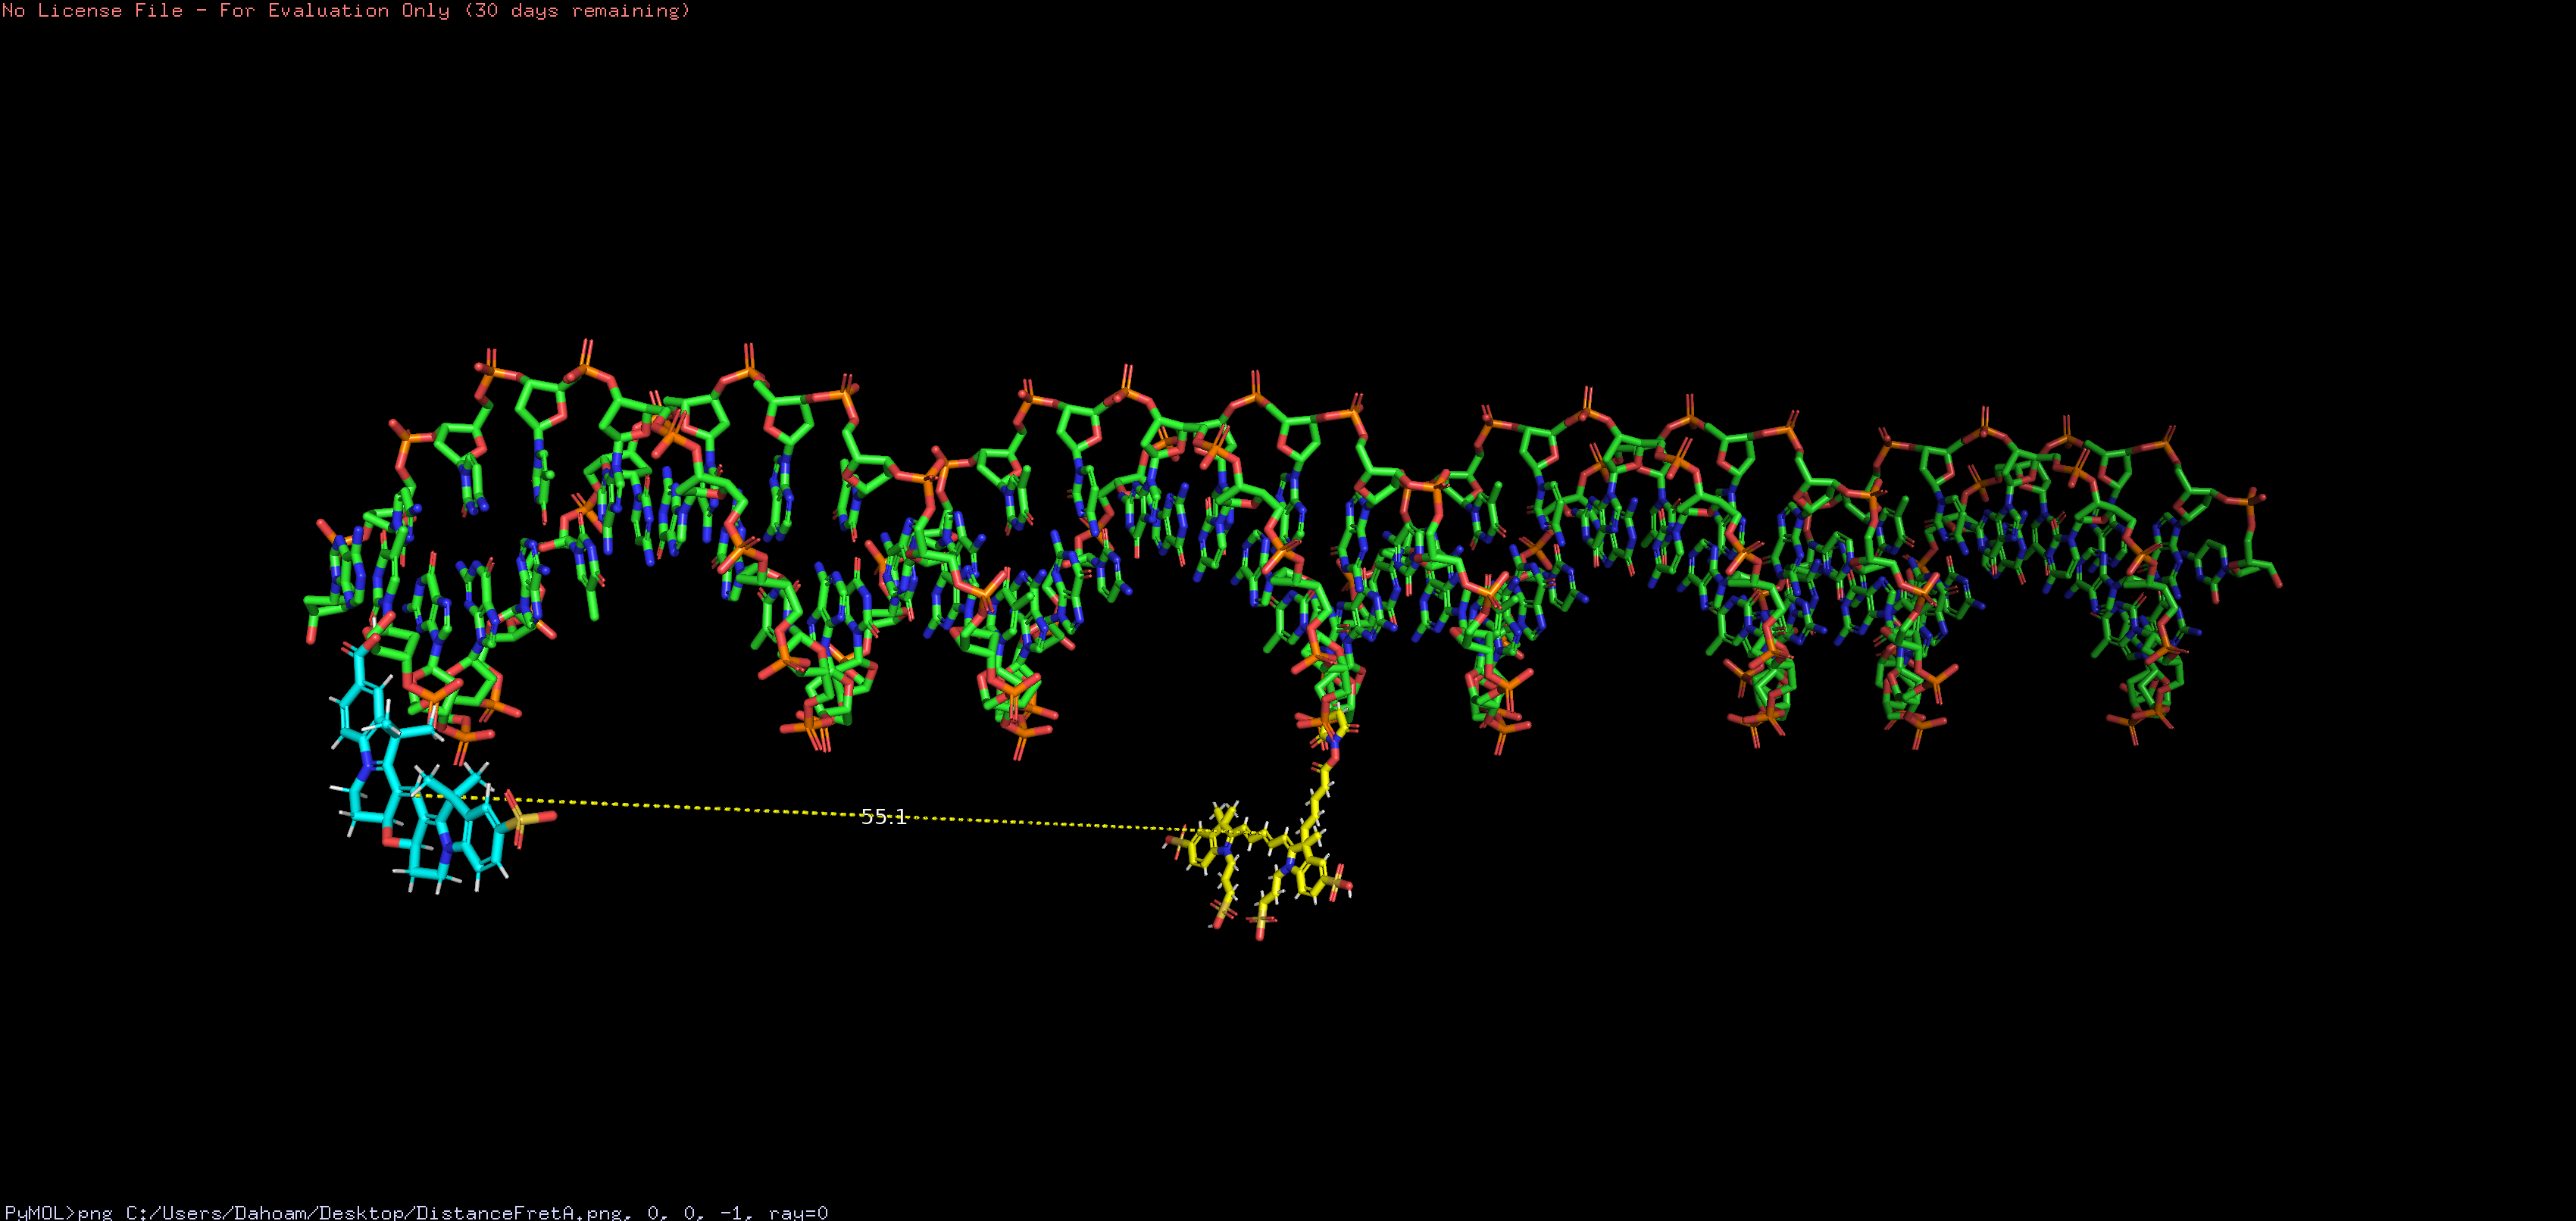
\includegraphics[width=0.8\textwidth]{images/other/DistanceFretA.png}
    \caption{simulated distance between donor and acceptor in FRET A}
    \label{Cy3_data1_fit1}
\end{figure}

\begin{figure}
    \centering
    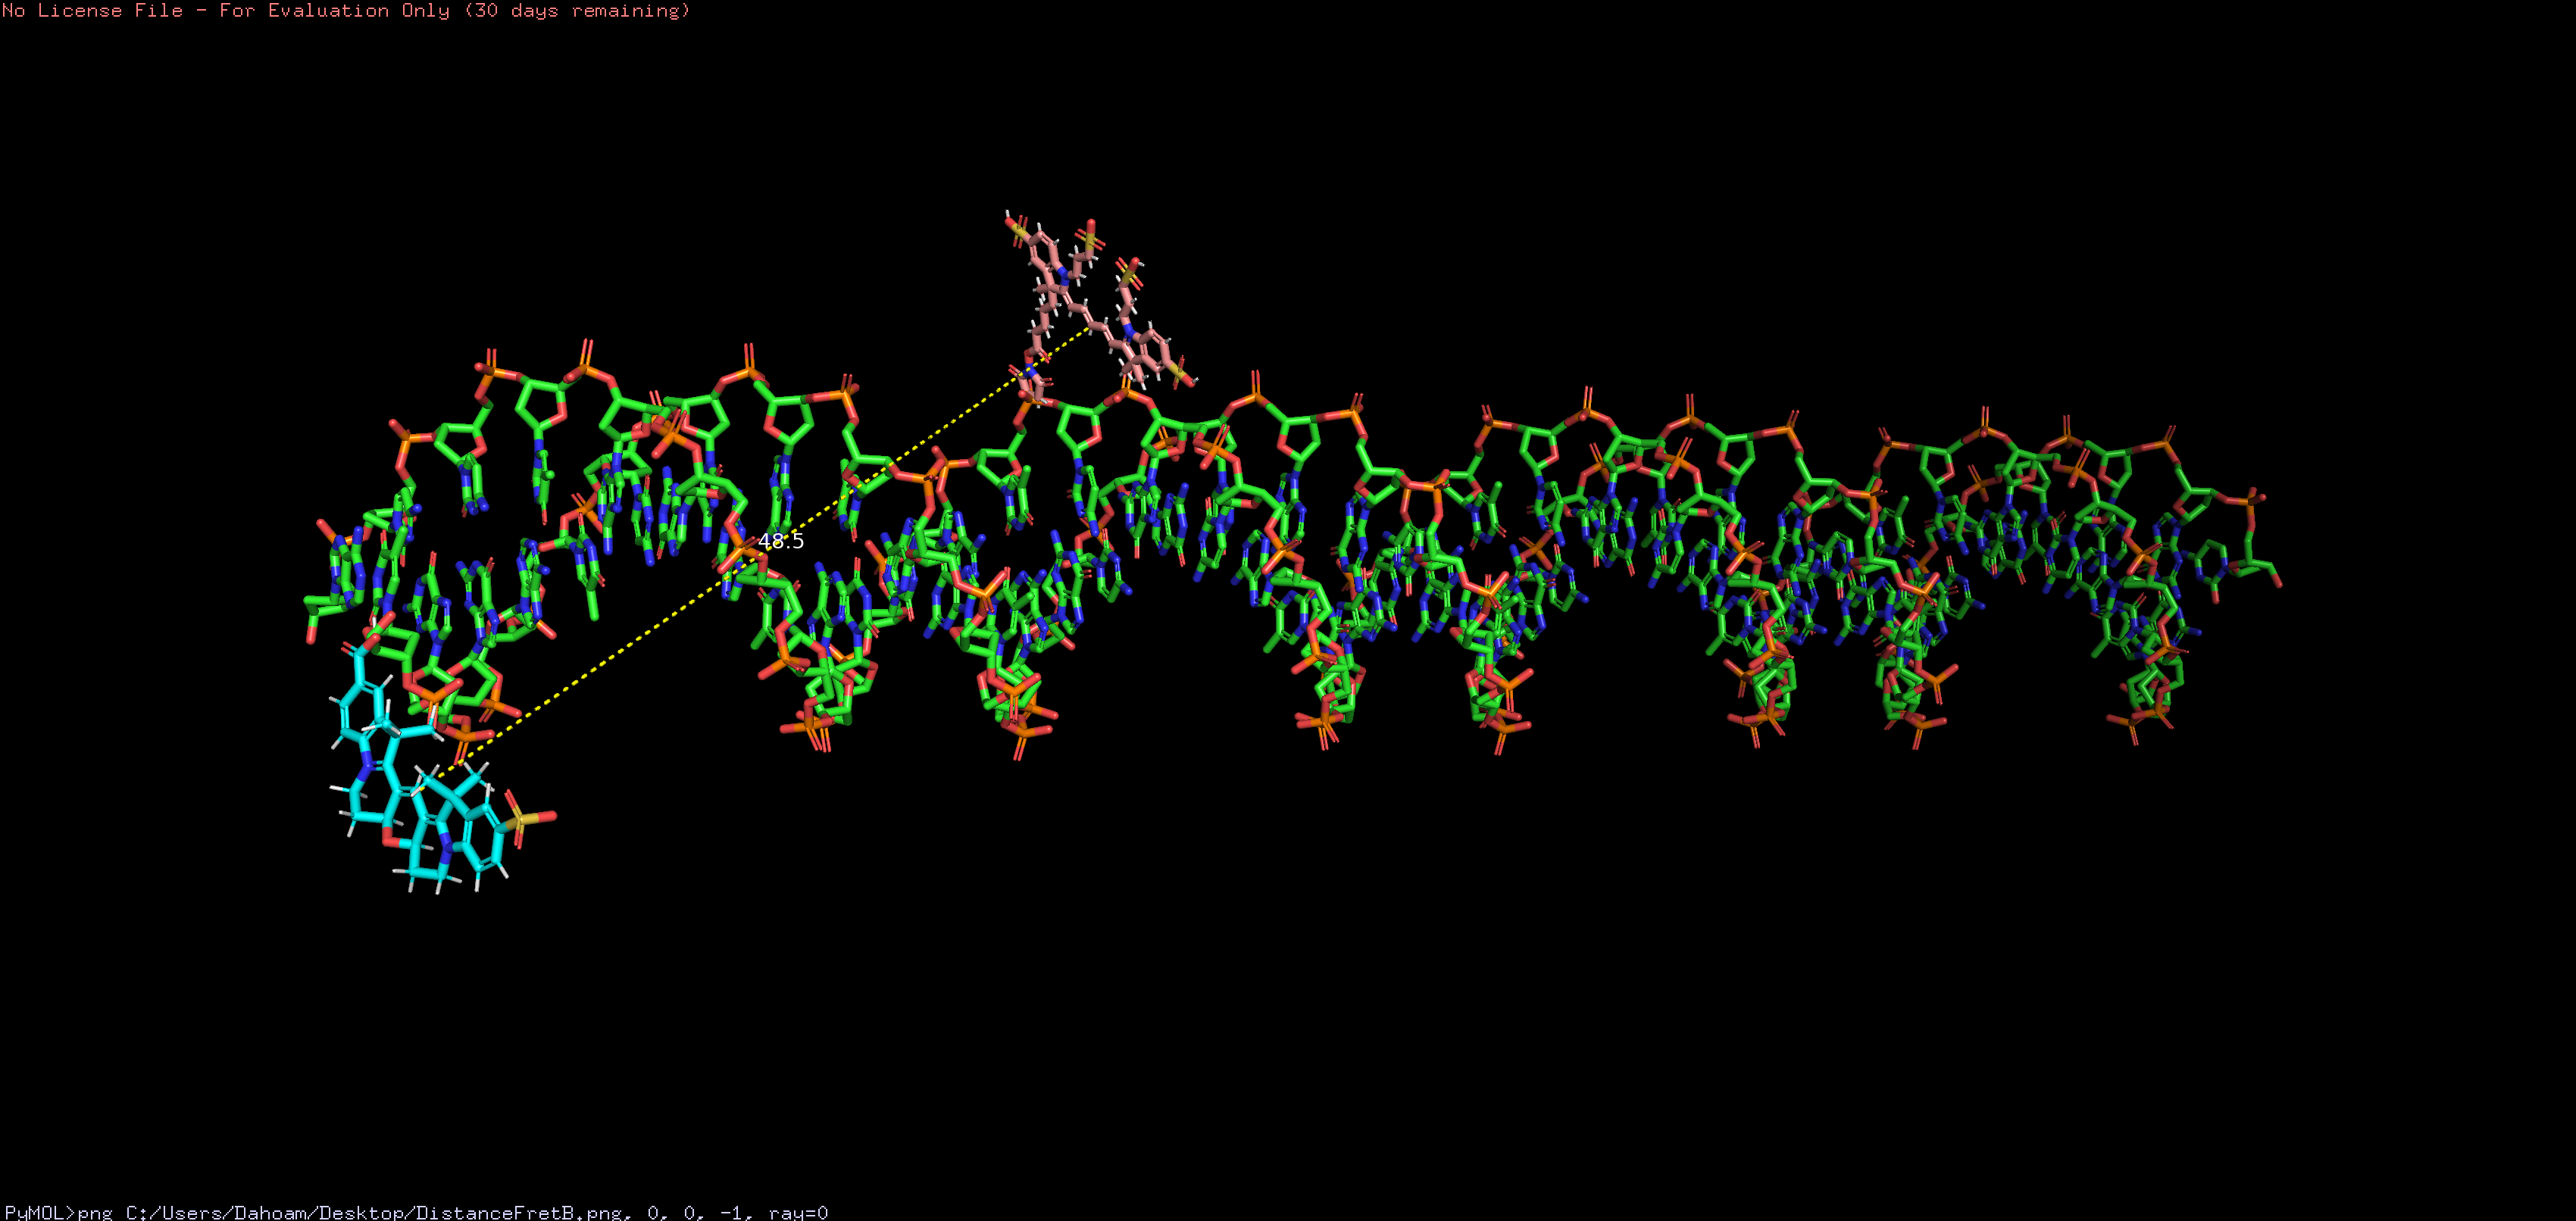
\includegraphics[width=0.8\textwidth]{images/other/DistanceFretB.png}
    \caption{simulated distance between donor and acceptor in FRET B}
    \label{Cy3_data1_fit1}
\end{figure}

\section{Discussion}
\label{sec:Discussion} 
In our fluorescence lifetime experiments, several key factors and considerations on sources of error should be taken into consideration for future replicates of this study. 
\\
Firstly, we had to consider the issues associated with the  Instrument Response Function (IRF), the IRF and real signal were recorded at 2 different wavelengths, from our perspective this can appear as an unreasonable approach in recording the IRF used to deconvolve the Photon Arrival Times of a different wavelength. However,this choice comes from the fact that the IRF is recorded with only PBS in the cuvette and for instance, at 500 nm you still get some signal, while at 570 nm, ( the wavelength used to record our arrival times) there is very low signal, making it unfeasible to record an IRF for each measurement in a reasonable amount of time. This could be due to the specific absorption and emission spectra of the Phosphate Buffer Solution itself which cannot be addressed in any way, as far as we know.\\
 
A second argument of discussion is the integrity of our samples, since we know that fluorescence lifetime is extremely sensitive to changes in the environment, particular attention should be given to consider how many possible fractions are contained in each sample. For instance samples containing just the Dye are actually composed of a fraction of fluorescing molecules with a specific average lifetime, and damaged molecules that do not fluoresce at all, and thus do not contribute to the measurement. This is ,in our opinion, the only true case where the TCSCP lifetime histogram can be explained by one single decay rate function. \\

In the case of more complex constructs, like the sample containing dsDNA-Cy3B , there can be multiple fractions, each contributing with their own average life time. For instance in a sample of seemingly pure dsDNA-Cy3 , there is a fraction of molecules which are ssDNA-Cy3 and display their own lifetime. We can argument that this molecules represent a fraction so insignificant that their contribution is lost to noise, but this argument stands on 2 principles: the first one is that the ssDNA-Cy3B and complementary ssDNA were reacted with perfectly stoichiometric amounts, and the second being that dsDNA is a static molecule, which we know that is actually better described as a dynamic equilibrium, in which Temperature and high energy photons have a major role.
\\
Considering our particular experiment, a notable mention should be given to the Cy3 Samples (Cy3, ssDNACy3, dsDNACy3) which regularly resulted in single fit exponential functions that have very high Chi-square, meaning that the single fit cannot explain a large part of our dataset.
This could be for the reasons stated above on the presence of multiple fractions, but assessing the likelihood of multiple fractions being present in the samples is beyond our analytical capabilities.
\\
However one could suggest that using the known lifetimes of previous recordings could potentially help improve the fit between the decay rate we are actually trying to record and the ones that we already have recordings for which make up the fractions of molecules contributing to the average lifetime as more noise that worsens the fit.\\

Moreover, replicates were essential in our experiments to account for variability in sample handling, and to increase the reliability of the results a greater amount of replicates( more than 3) should be considered. Longer recordings can also lead to  a smoother TCSCP histogram, improving fitting results even further. All of the above mentioned techniques come at the price of time and reagents.\\

Considering the usage of PyMOL to estimate FRET pair distance, we need to state that it was used in a rudimentary way, thus creating rudimentary results. The orientation of the dyes and the distances between FRET pairs may not be significant from a molecular standpoint  because they were not the result of a molecular simulation, but just from manipulations on the known structures of the DNA and dye molecules.\\
Lastly, variability in measurement times could be attributed to several factors, including low concentration of the sample caused by inefficient drying of the cuvette or altered quantum efficiency of the dyes. These factors can affect the time spent for each measurement and lead to variability in the measurements.\\

\chapter{Conclusion}
\label{cha:Conclusion}
In this experiment, we applied the fluorescence lifetime measuring by time-correlated single photon counting(TCSPC). Single and double exponential fitting were used to acquire the fluorescence lifetime. We conducted the TCSPC on Cy3 PBS solution, Cy3B PBS solution, Cy3 labeled single-stranded DNA, Cy3B labeled single-stranded DNA, Cy3 labeled double-stranded DNA, Cy3B labeled double-stranded DNA, FRET A and FRET B. For each group, the fluorescence lifetime is at reasonable values (compared with typical values). Furthermore, we calculated the energy transfer efficiency, relative amplitude, and donor-acceptor distance for the FRET A and FRET B samples, and acquired good experimental results comparable to the theoretical values.

\chapter{Appendix}
\label{cha:Appendix}

All the TCSPC curves obtained in the experiment are in the appendix.
\begin{figure}
    \centering
    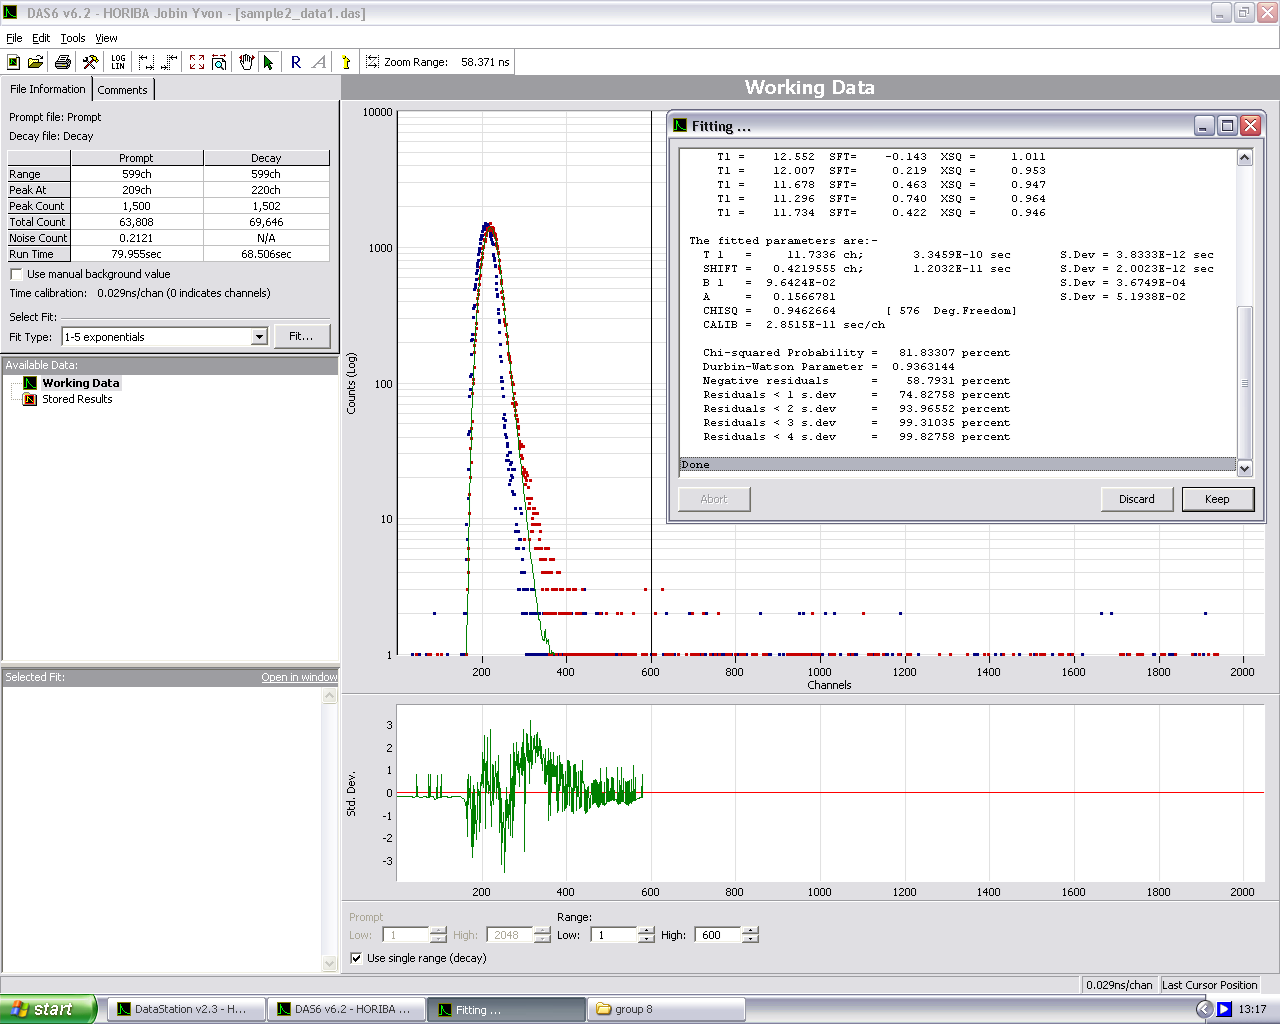
\includegraphics[width=0.8\textwidth]{images/dyes/Cy3_data1_fit1.png}
    \caption{TCSPC curve and the fitting of the first replicate of Cy3}
    \label{Cy3_data1_fit1}
\end{figure}

\begin{figure}
    \centering
    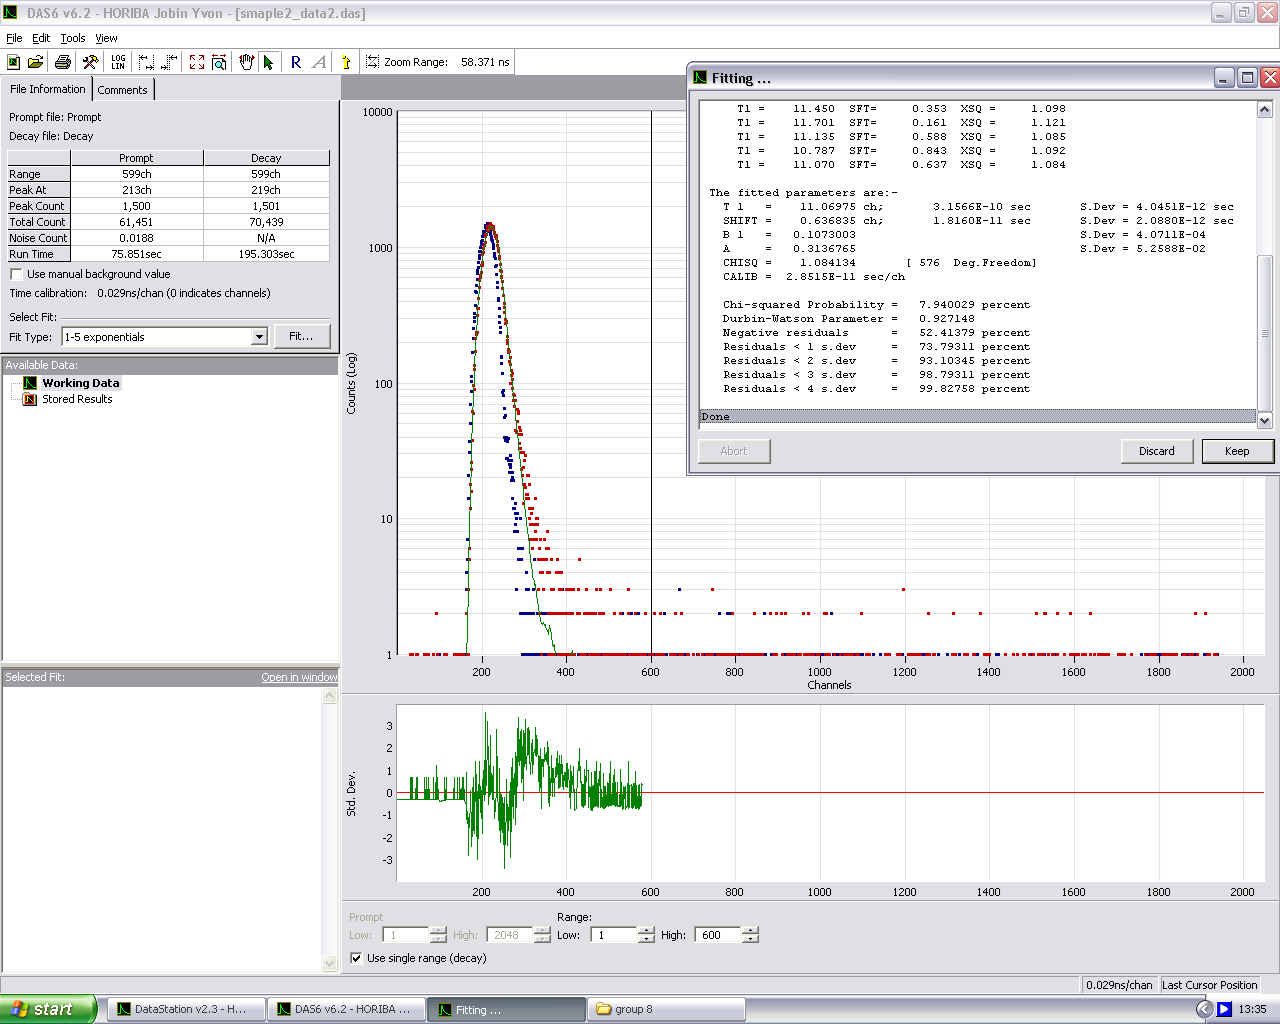
\includegraphics[width=0.8\textwidth]{images/dyes/Cy3_data2_fit1.png}
    \caption{TCSPC curve and the fitting of the second replicate of Cy3}
    \label{Cy3_data2_fit1}
\end{figure}

\begin{figure}
    \centering
    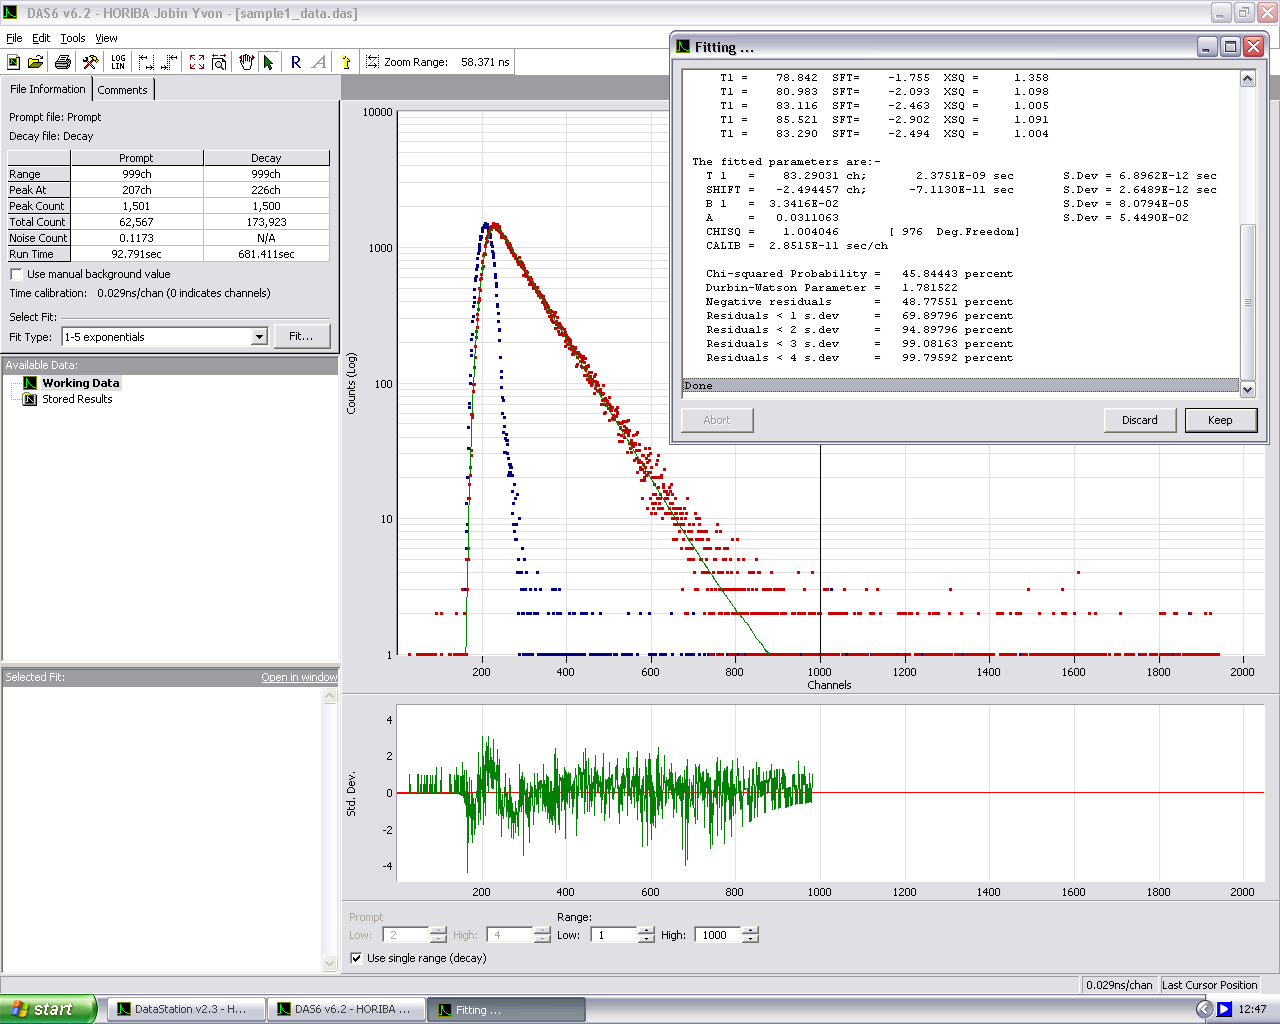
\includegraphics[width=0.75\textwidth]{images/dyes/Cy3B_fit1.png}
    \caption{TCSPC curve and the fitting of the Cy3B}
    \label{Cy3B_data1_fit1}
\end{figure}

\begin{figure}
    \centering
    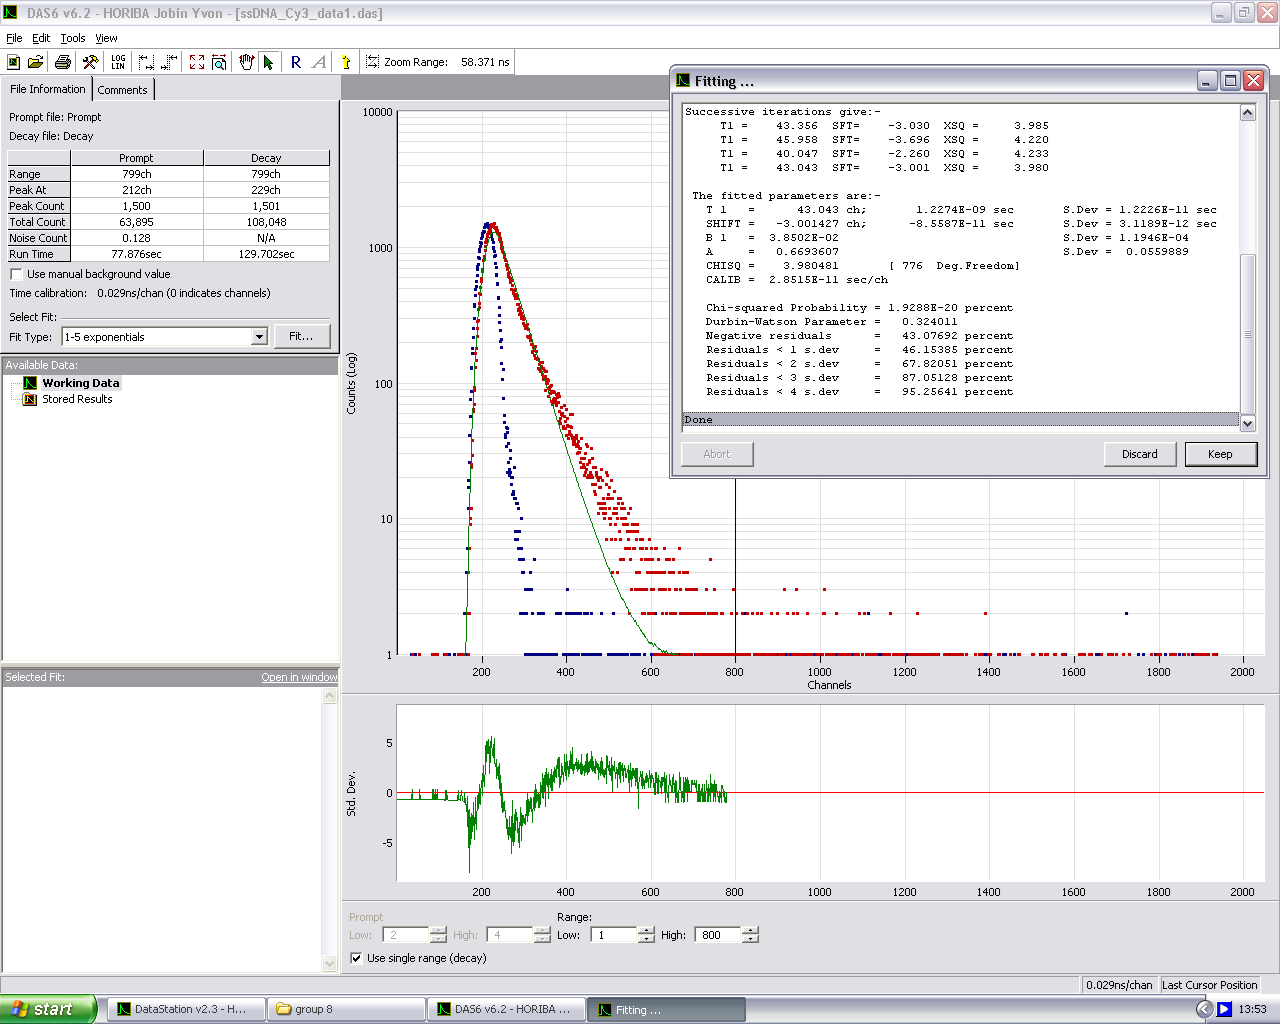
\includegraphics[width=0.75\textwidth]{images/ssDNA/ssDNA_Cy3_data1_fit1.png}
    \caption{TCSPC curve and the fitting of the first replicate of 5'-Cy3-labeled single-stranded DNA}
    \label{ssDNA_Cy3_data1_fit1}
\end{figure}

\begin{figure}
    \centering
    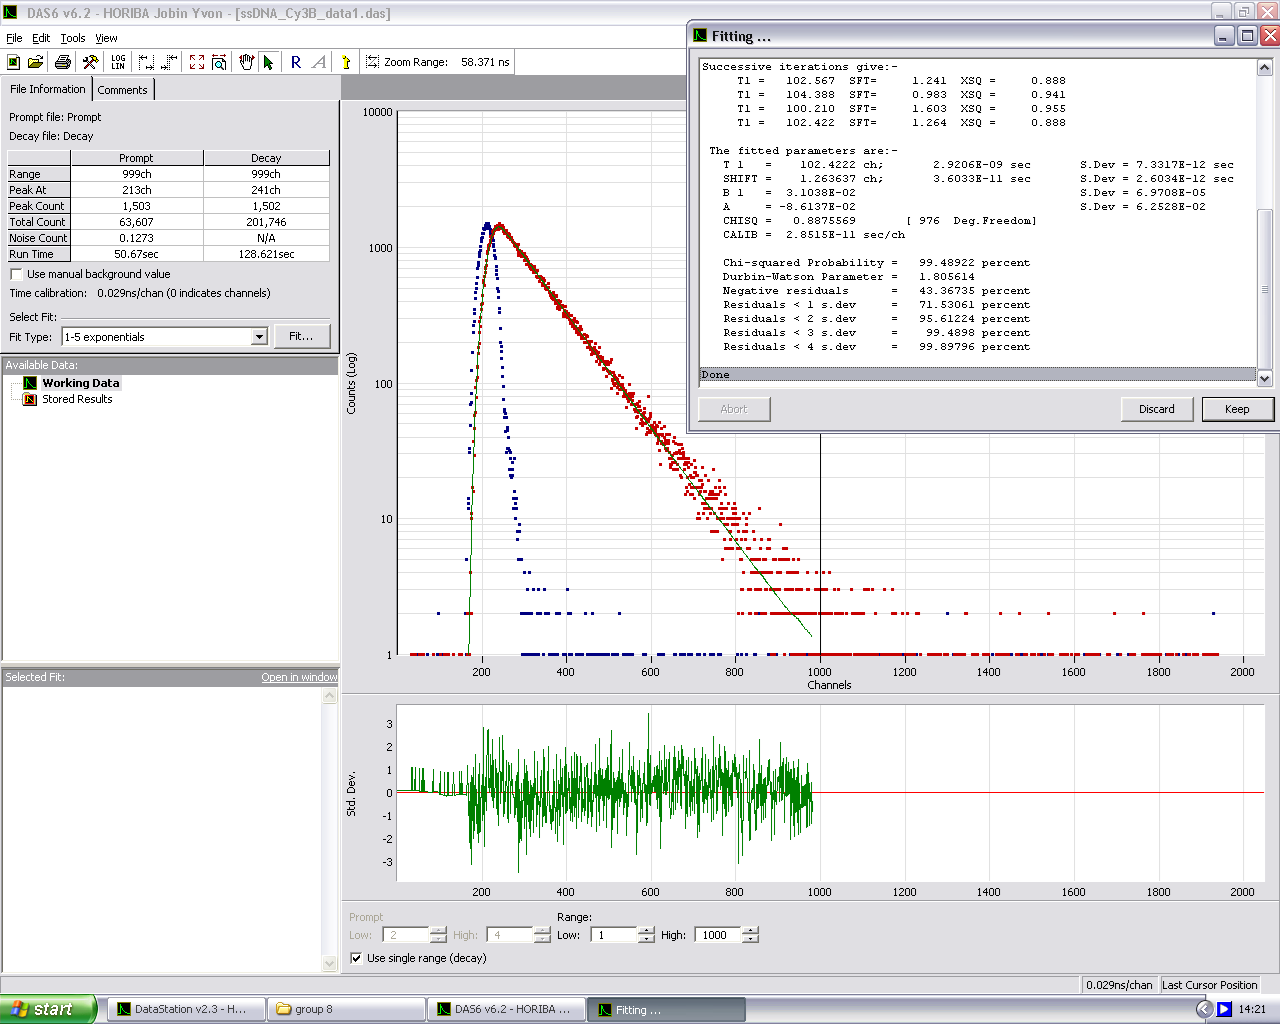
\includegraphics[width=0.75\textwidth]{images/ssDNA/ssDNA_Cy3B_data1_fit1.png}
    \caption{TCSPC curve and the fitting of the first replicate of Cy3B-labeled single-stranded DNA}
    \label{Cy3B_data1_fit1}
\end{figure}

\begin{figure}
    \centering
    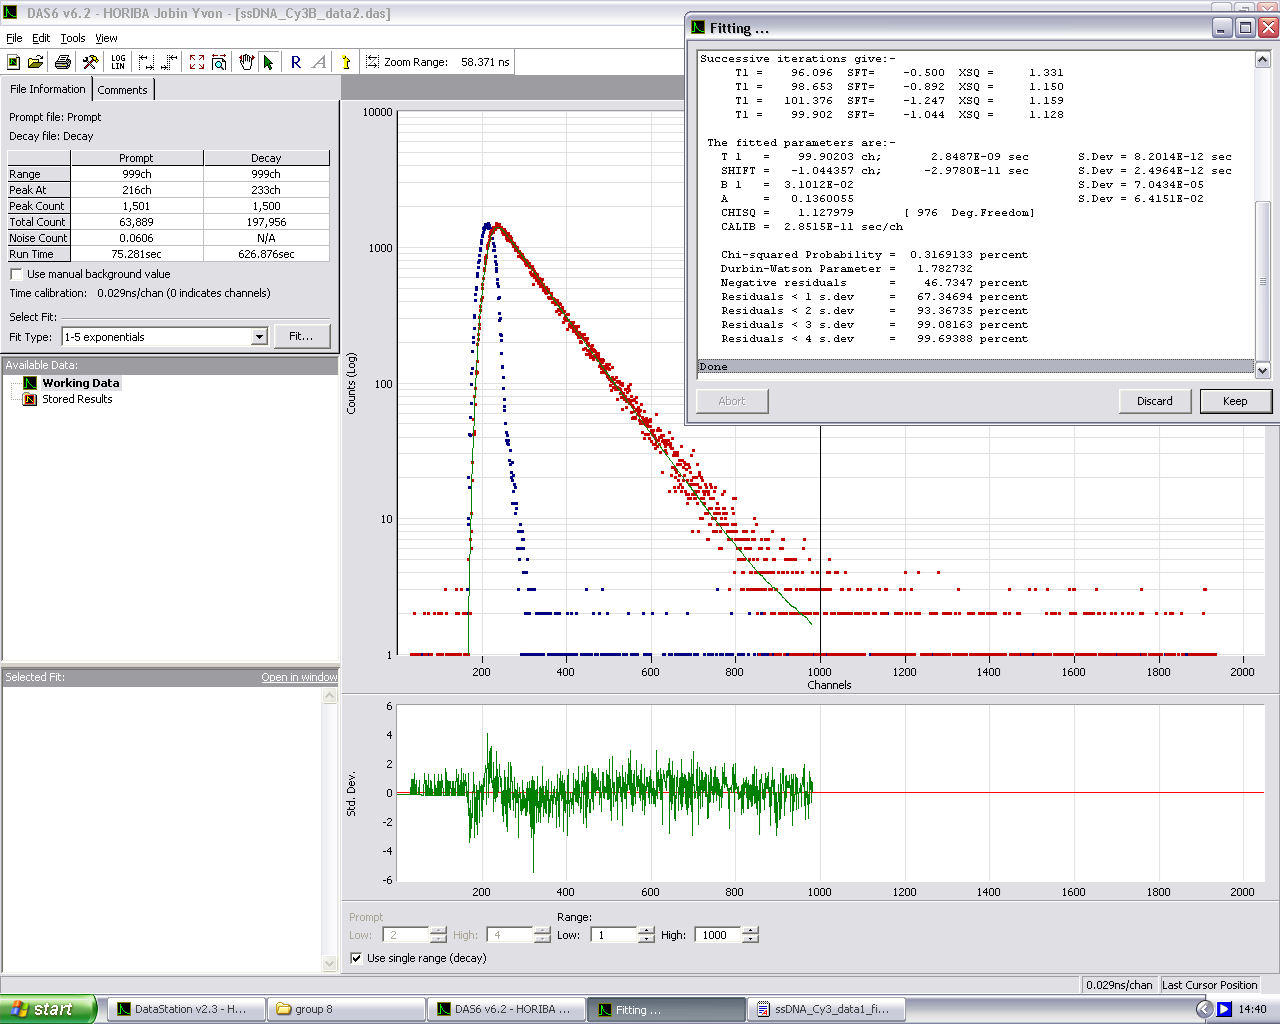
\includegraphics[width=0.75\textwidth]{images/ssDNA/ssDNA_Cy3B_data2_fit1.png}
    \caption{TCSPC curve and the fitting of the second replicate of Cy3B-labeled single-stranded DNA}
    \label{Cy3B_data2_fit1}
\end{figure}

\begin{figure}
    \centering
    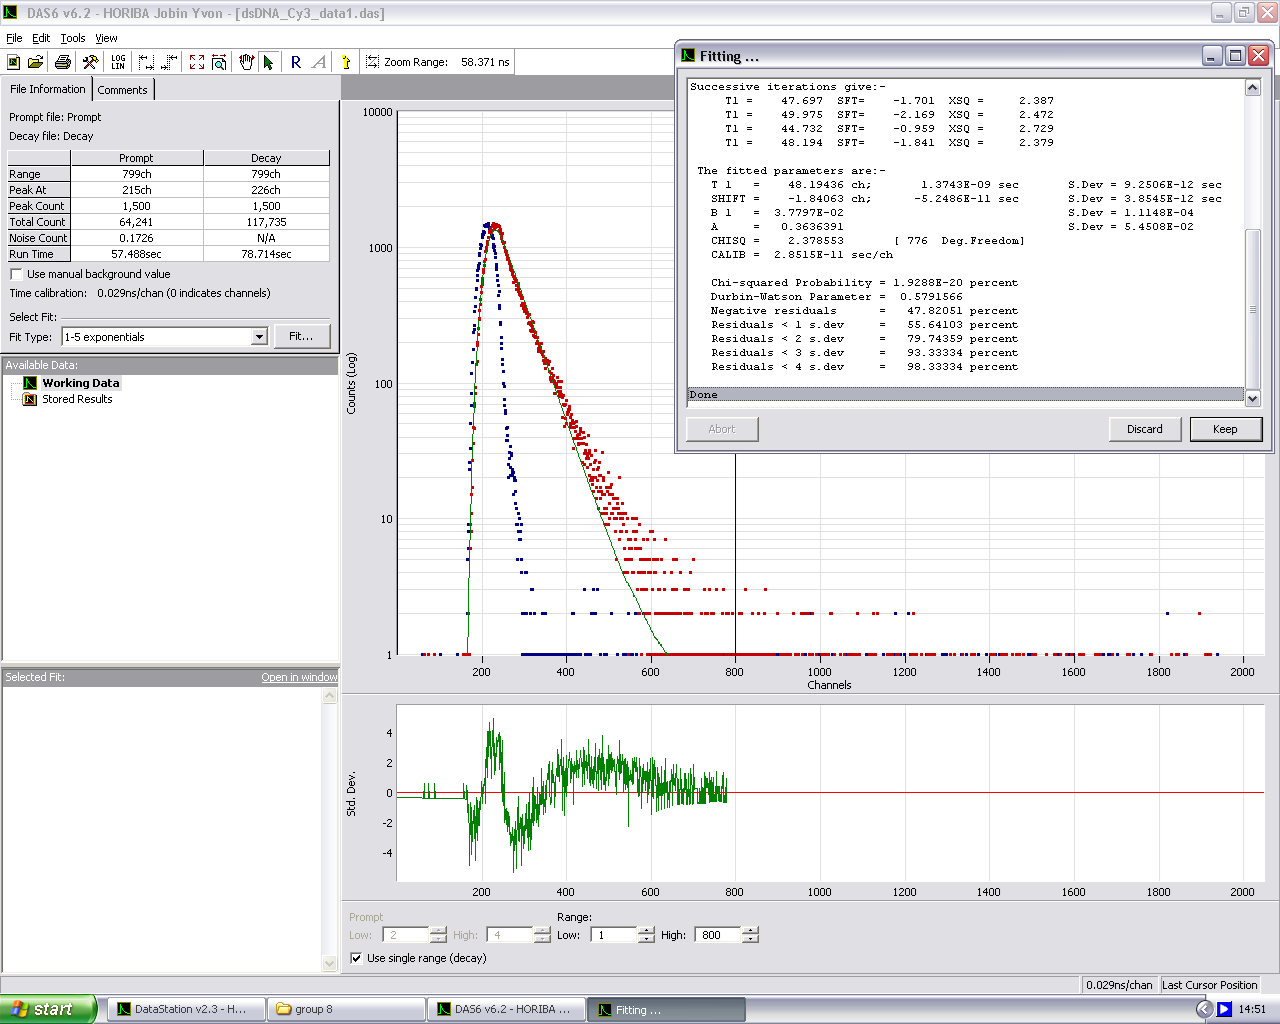
\includegraphics[width=0.75\textwidth]{images/dsDNA/dsDNA_Cy3_data1_fit1.png}
    \caption{TCSPC curve and the fitting of the first replicate of Cy3-labeled double-stranded DNA}
    \label{dsDNA_Cy3_data1_fit1}
\end{figure}

\begin{figure}
    \centering
    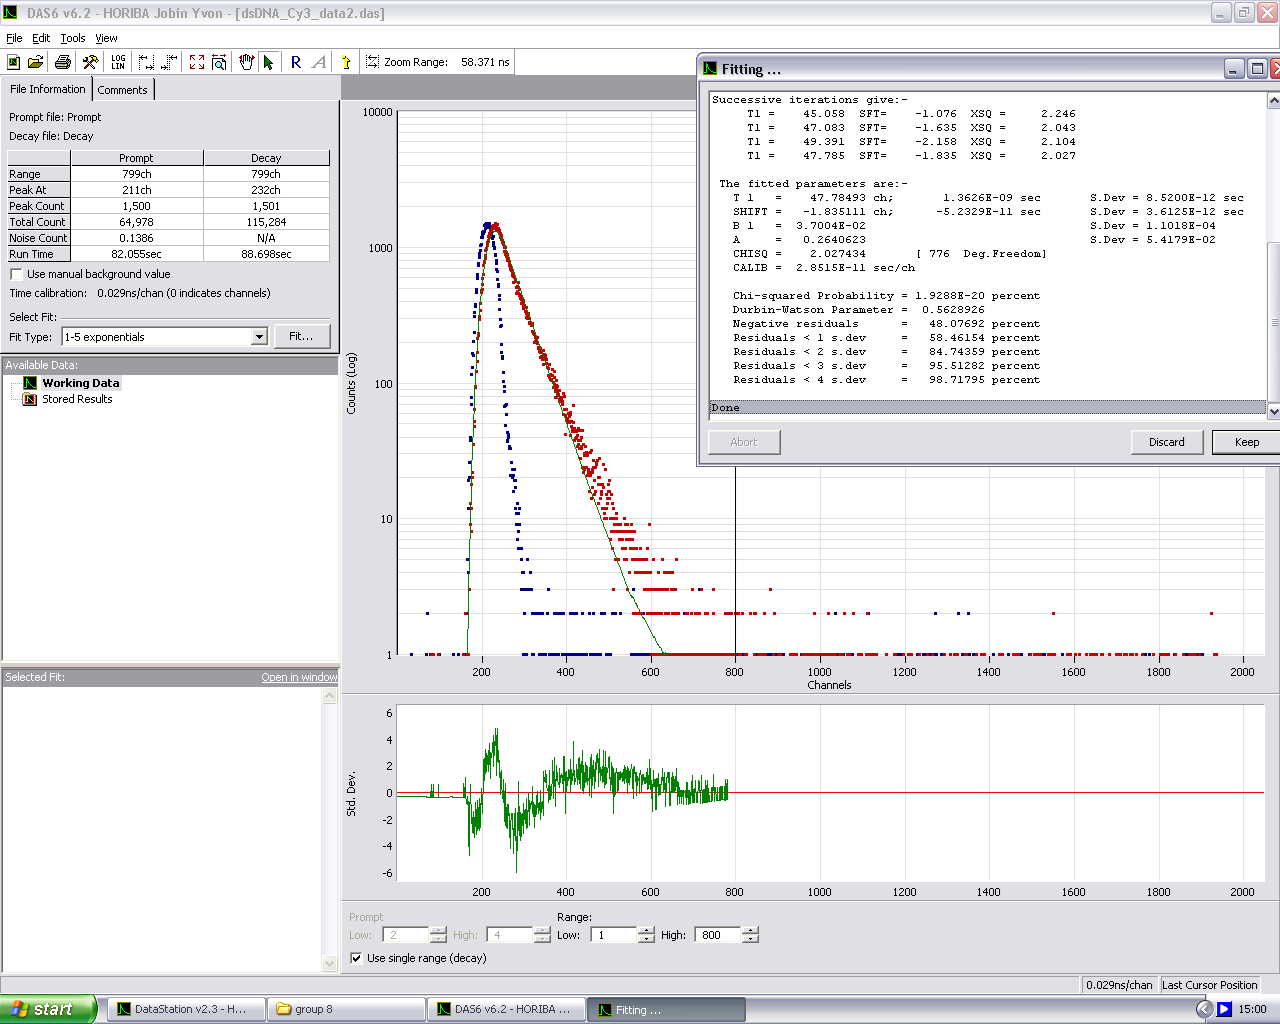
\includegraphics[width=0.75\textwidth]{images/dsDNA/dsDNA_Cy3_data2_fit1.png}
    \caption{TCSPC curve and the fitting of the second replicate of Cy3-labeled double-stranded DNA}
    \label{dsDNA_Cy3_data2_fit1}
\end{figure}

\begin{figure}
    \centering
    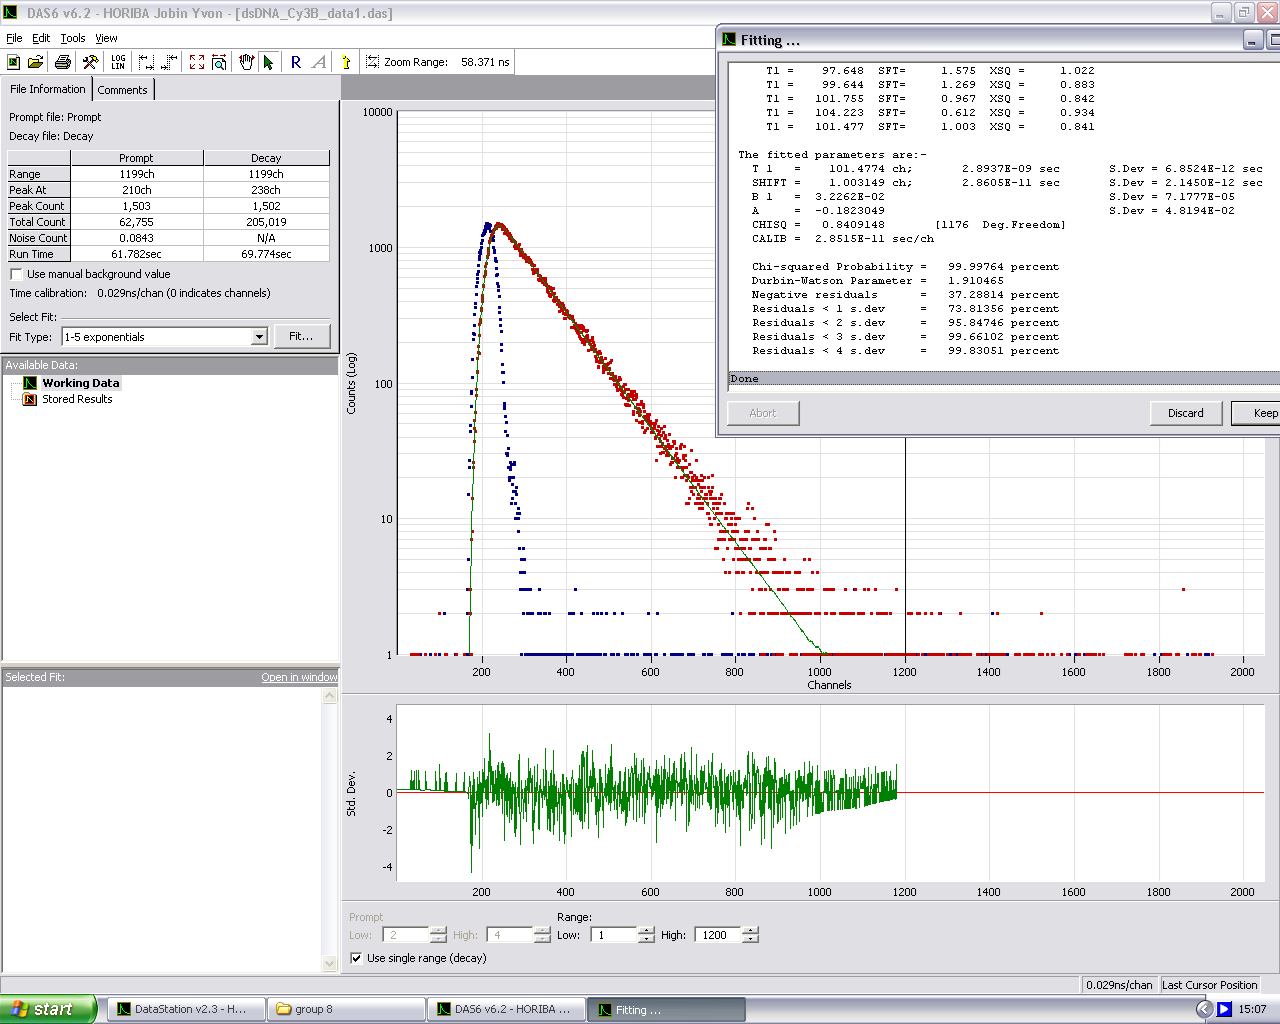
\includegraphics[width=0.75\textwidth]{images/dsDNA/dsDNA_Cy3B_data1_fit1.png}
    \caption{TCSPC curve and the fitting of the first replicate of Cy3B-labeled double-stranded DNA}
    \label{dsDNA_Cy3B_data1_fit1}
\end{figure}

\begin{figure}
    \centering
    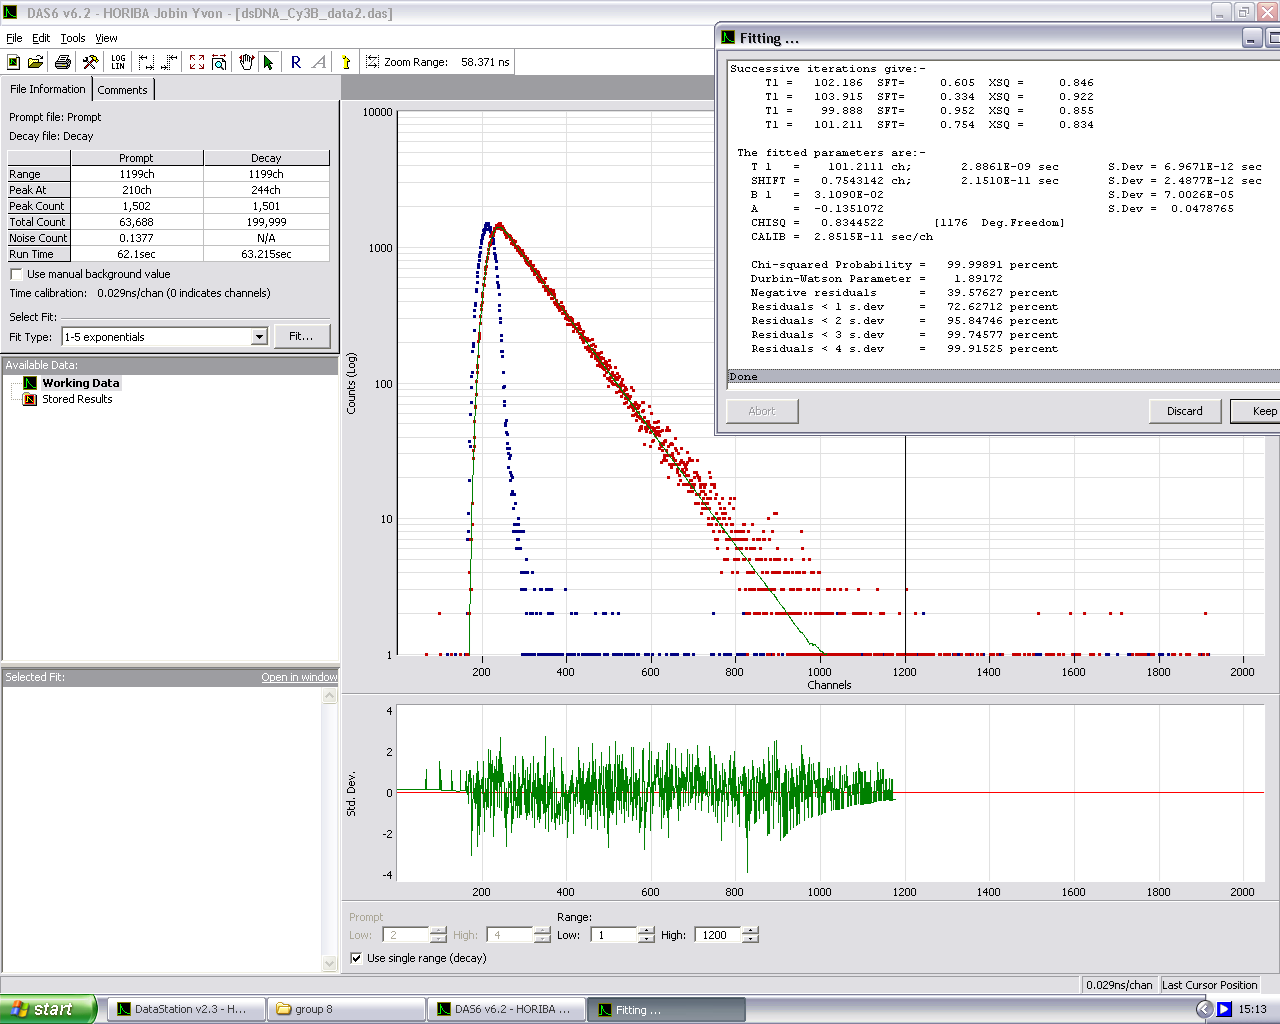
\includegraphics[width=0.75\textwidth]{images/dsDNA/dsDNA_Cy3B_data2_fit1.png}
    \caption{TCSPC curve and the fitting of the second replicate of Cy3B-labeled double-stranded DNA}
    \label{dsDNA_Cy3B_data2_fit1}
\end{figure}

\begin{figure}
    \centering
    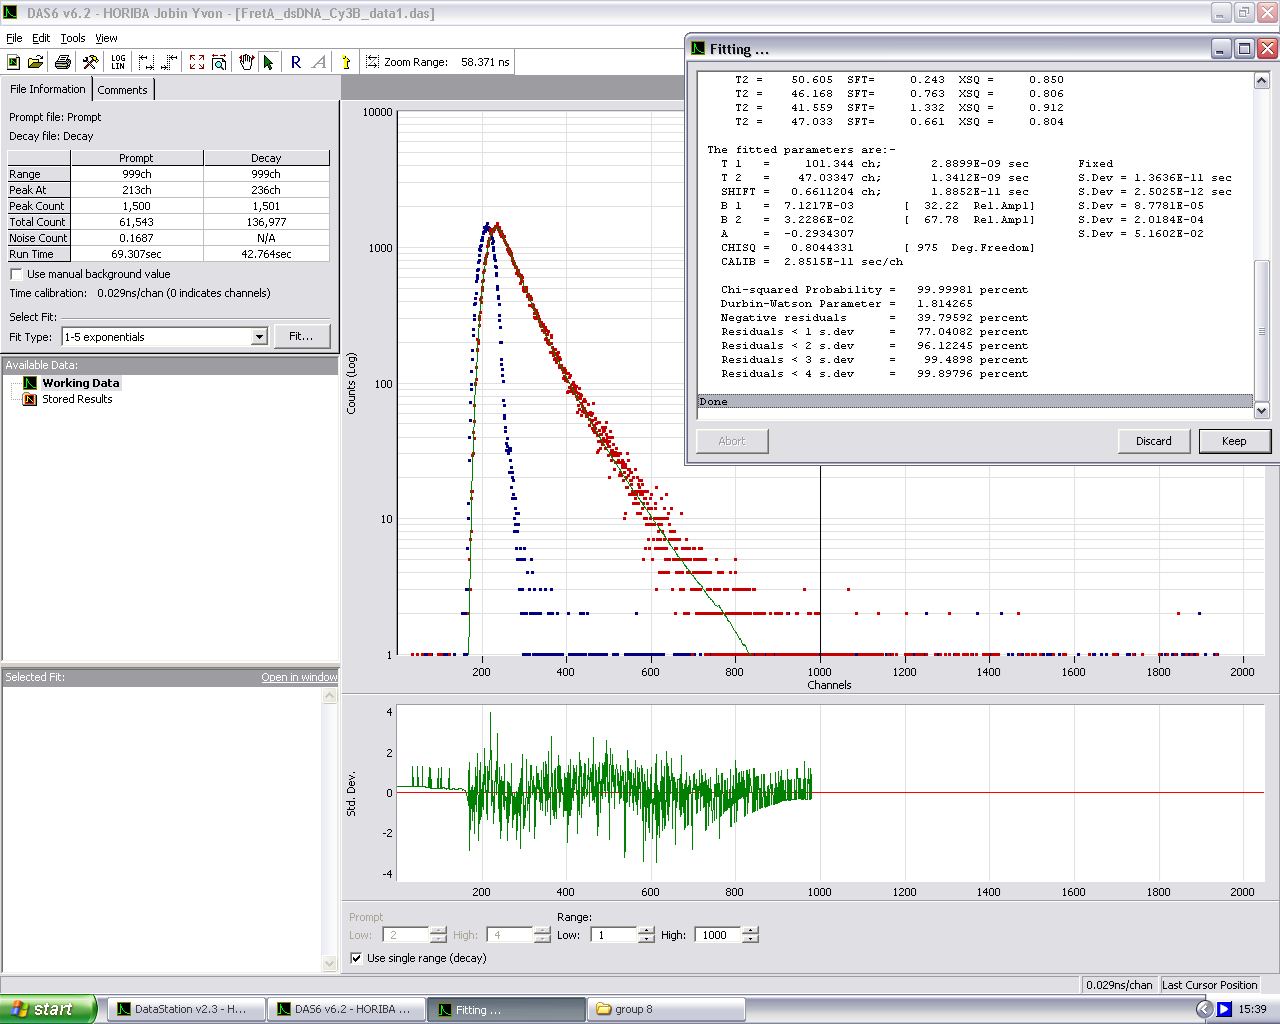
\includegraphics[width=0.75\textwidth]{images/FRET/FretA_dsDNA_Cy3B_data1_fit2.png}
    \caption{TCSPC curve and the fitting of the first replicatep of FRET A sample}
    \label{FretA_dsDNA_Cy3B_data1}
\end{figure}

\begin{figure}
    \centering
    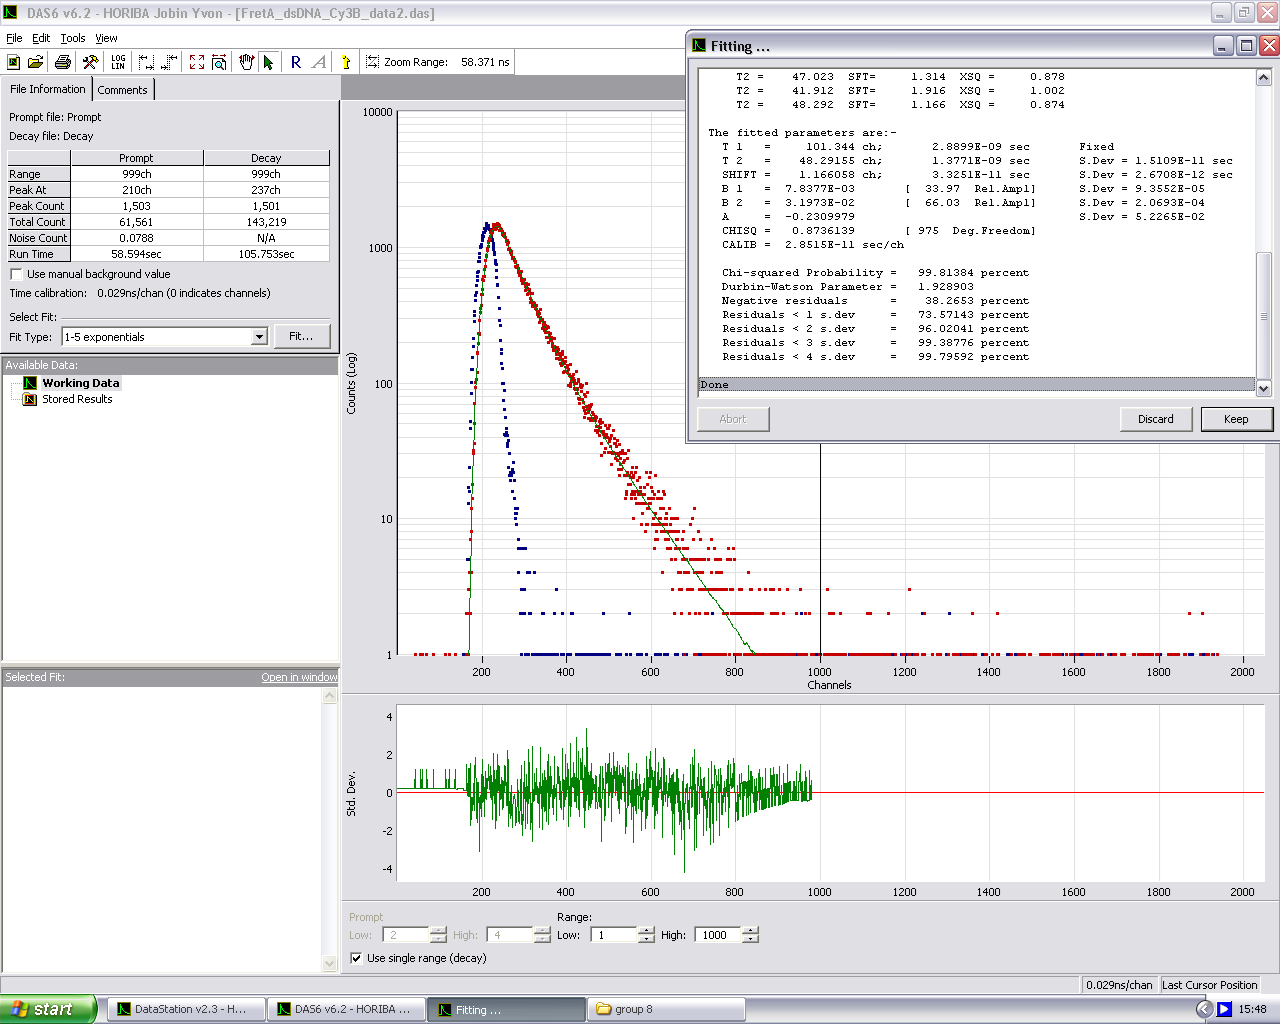
\includegraphics[width=0.75\textwidth]{images/FRET/FretA_dsDNA_Cy3B_data2_fit2.png}
    \caption{TCSPC curve and the fitting of the second replicate of FRET A sample}
    \label{FretA_dsDNA_Cy3B_data2}
\end{figure}

\begin{figure}
    \centering
    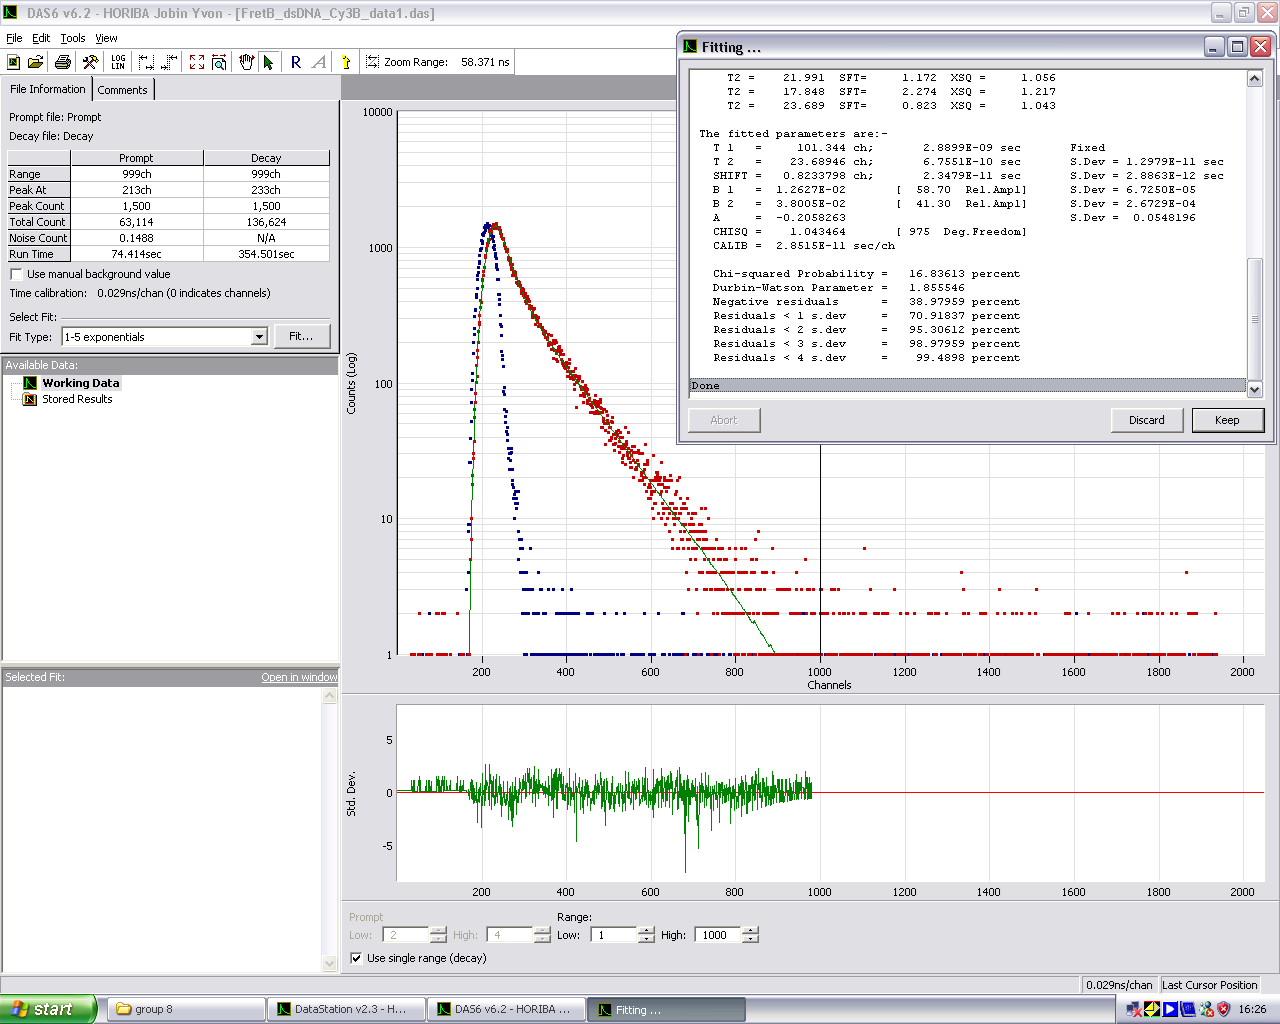
\includegraphics[width=0.75\textwidth]{images/FRET/FretB_dsDNA_Cy3B_data1_fit2.png}
    \caption{TCSPC curve and the fitting of the first replicate of FRET B sample}
    \label{FretB_dsDNA_Cy3B_data1_fit2}
\end{figure}

\begin{figure}
    \centering
    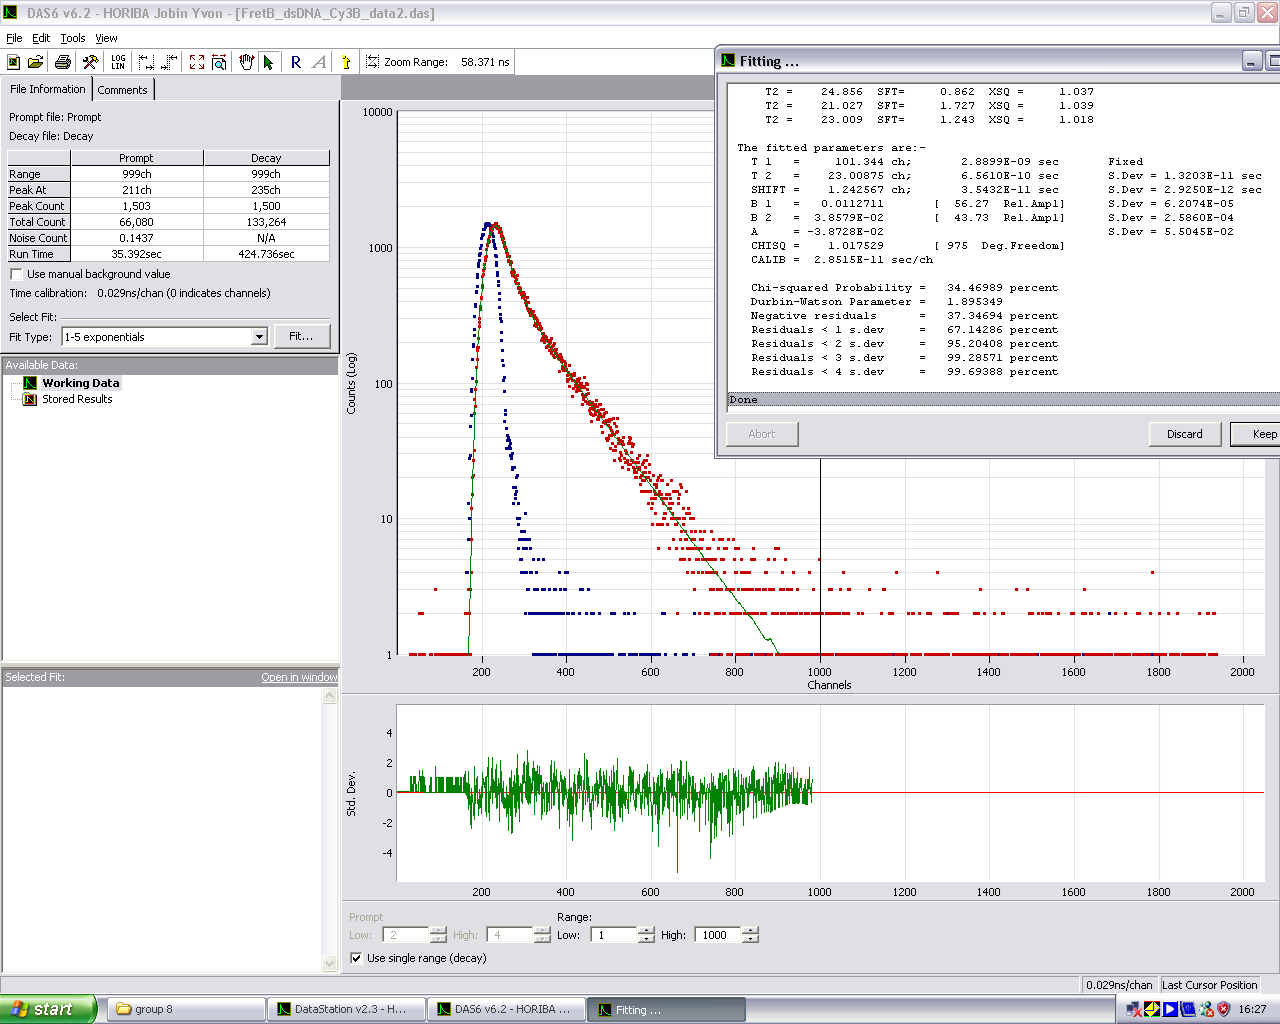
\includegraphics[width=0.75\textwidth]{images/FRET/FretB_dsDNA_Cy3B_data2_fit2.png}
    \caption{TCSPC curve and the fitting of the second replicate of FRET B sample}
    \label{FretB_dsDNA_Cy3B_data2_fit2}
\end{figure}


\chapter{References}
\label{cha:References}

[1]\label{sec:ref_1}: Lakowicz, J.R. (1999). Introduction to Fluorescence. In: Principles of Fluorescence Spectroscopy. Springer, Boston, MA. https://doi.org/10.1007/978-1-4757-3061-6\_1\\

[2]\label{sec:ref_2}: Jablonski diagram, wikipedia, https://en.wikipedia.org/wiki/Jablonski\_diagram\\

[3]\label{sec:ref_3}: Fluorescence lifetime, Biophysics lab course, Ulm University.\\

[4]\label{sec:ref_4}: Spectrum [Cy3 (Cyanine-3)], AAT Bioquest, https://www.aatbio.com/fluorescence-excitation-emission-spectrum-graph-viewer/cy3\_cyanine\_3\\

[5]\label{sec:ref_5}: PyMOL, The PyMOL Molecular Graphics System, Version 1.8, Schr{\"o}dinger, LLC. 2015


\end{document}